\documentclass{beamer}
% % Example from http://www.math.umbc.edu/~rouben/beamer/quickstart-Z-H-3.html#node_sec_3
%\usepackage{default}
\usetheme{default}
\usepackage{hyperref}
\usepackage[utf8]{inputenc}  % this allows latex to understand UTF
                             % encoding in the file. This is
                             % important for Icelandic characters.
\usepackage[T1]{fontenc} % this enables icelandic characters in the output

\usepackage[caption=false]{subfig}

% % Use the UMBC theme
% Template derived from hfc.tex by
% Rouben Rostamian <rostamian@umbc.edu>
% August 31, 2004 
\usetheme{ru1}
\useinnertheme{ruboxes}
\setbeamercolor{ruboxes}{bg=violet!12,fg=black}

\usepackage{rotating} % for defining \schwa
\newcommand{\schwa}{\raisebox{1ex}{\begin{turn}{180}e\end{turn}}}

\title{GeoLog "Data Collector"}
\subtitle{Final Project Presentation}
\author[P. Helgasson, S. Ólafsson, S. Magnússon, \& Þ. Tómasarson]{Páll Helgason pallsh12@ru.is, Sindri Ólafsson sindrio12@ru.is, Sveinn Elmar Magnússon sveinnm12@ru.is, \& Þór Tómasarson thortom12@ru.is}
\institute[RU]{
  Department of Science and Engineering (TVD) \\
  Reykjavík University \\
}
\date{November 6, 2014} %% Put the real presentation day so it doesn't
                        %% change later
\begin{document}

%----------- titlepage ----------------------------------------------%
\begin{frame}[plain]
  \titlepage
\end{frame}

%----------- slides ----------------------------------------------%
\begin{frame}{Introduction}
	\begin{itemize}
	% sett each as seperate slide...
	\item Geological data collector
	\item Collects data from multiple sensors and sends the data over the world wide web. 
	\item Eases the observation of wide terrain
	\end{itemize}
	\begin{figure}
			\centering
	        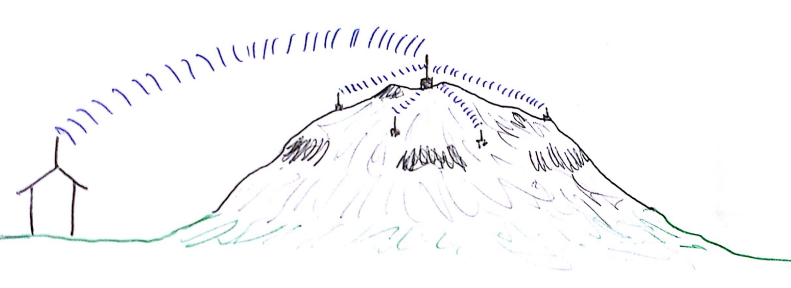
\includegraphics[height=3cm]{graphics/GeoLog.PNG}
	        \caption{Datalogging}
	\end{figure}
\end{frame}

\begin{frame}{Introduction}
\begin{itemize}
\item Andrew D. Wickert cares.
\end{itemize}
\centering
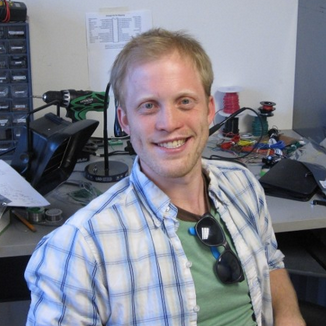
\includegraphics[height=5cm]{graphics/andrewWickert.png}
\cite{andrewWickert}
\end{frame}

\begin{frame}{Andy's Andrew D. Wickert}
\begin{figure}
\centering
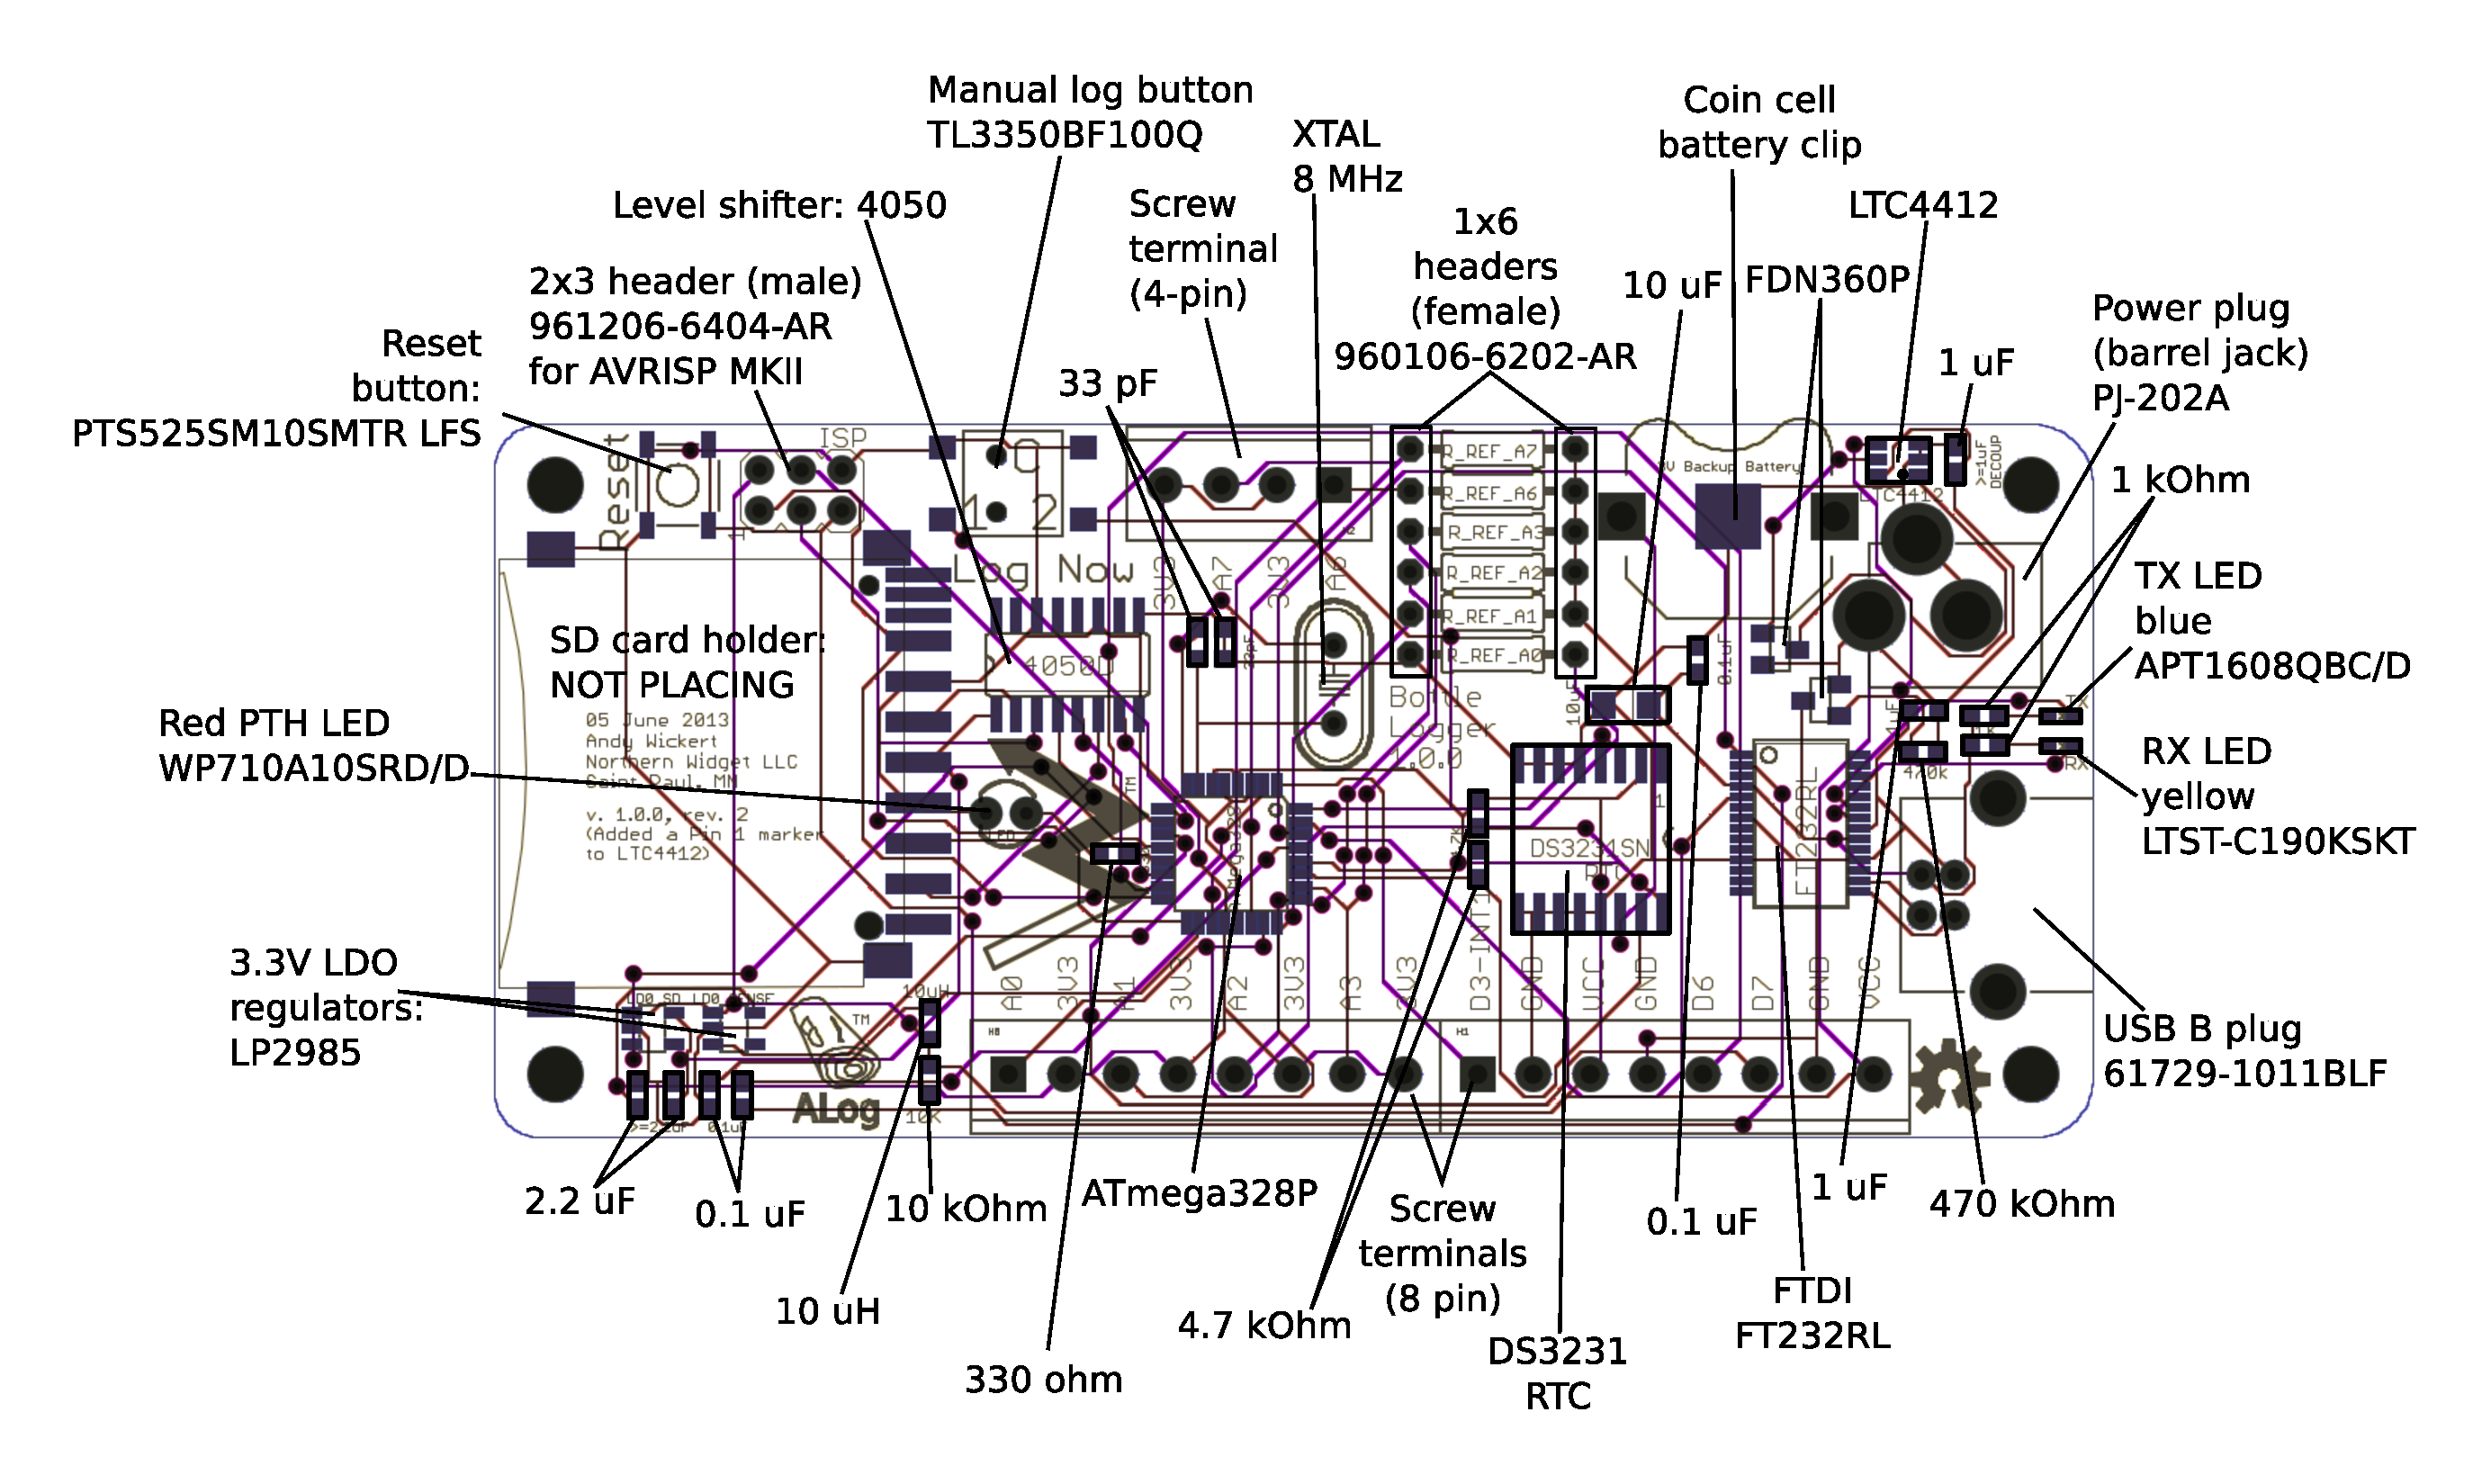
\includegraphics[height=5.7cm]{graphics/ALog_drawing.PDF}
\caption{Arduino-based low-power field environmental data logging platform: hardware schematics and circuit board layouts\cite{ALog-BottleLogger}}

\end{figure}
\end{frame}

\begin{frame}{Similar products}
\begin{figure}
  \centering
  \subfloat[\$3500\label{fig:a}\cite{WeatherShop2014}]
  {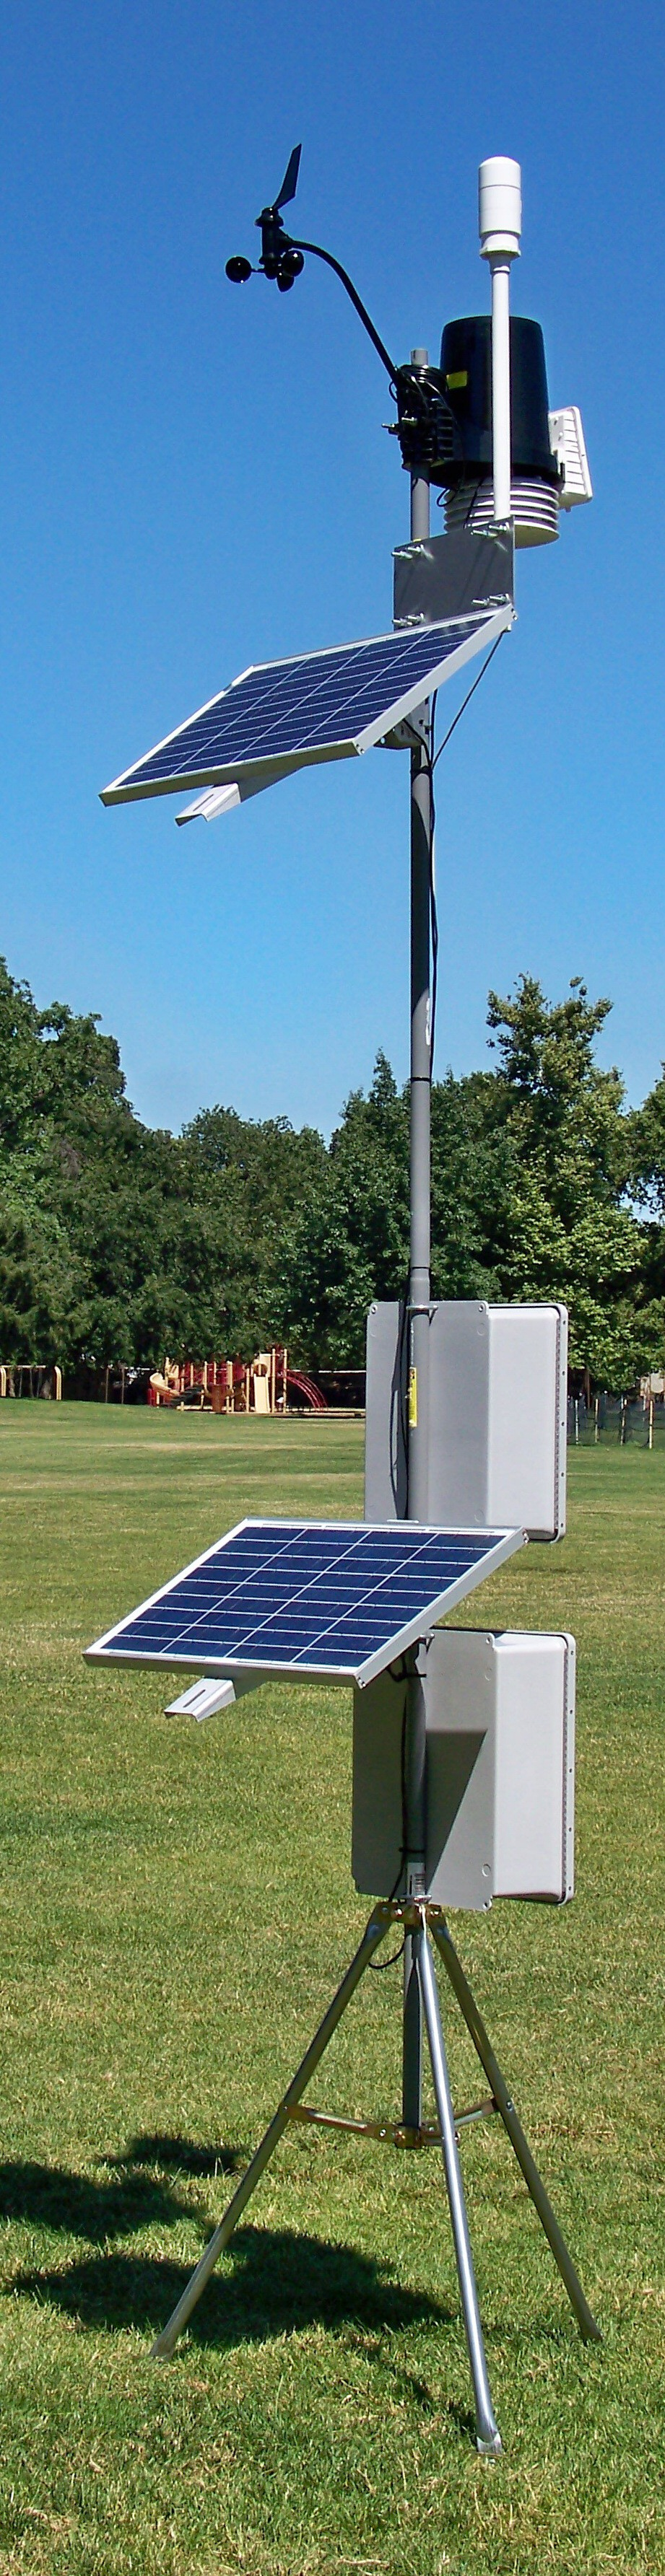
\includegraphics[height=5cm]{graphics/cellular_weather_station.JPG}}\quad
  \subfloat[\$2800\label{fig:b}\cite{TexasWeatherInstruments2014}]
  {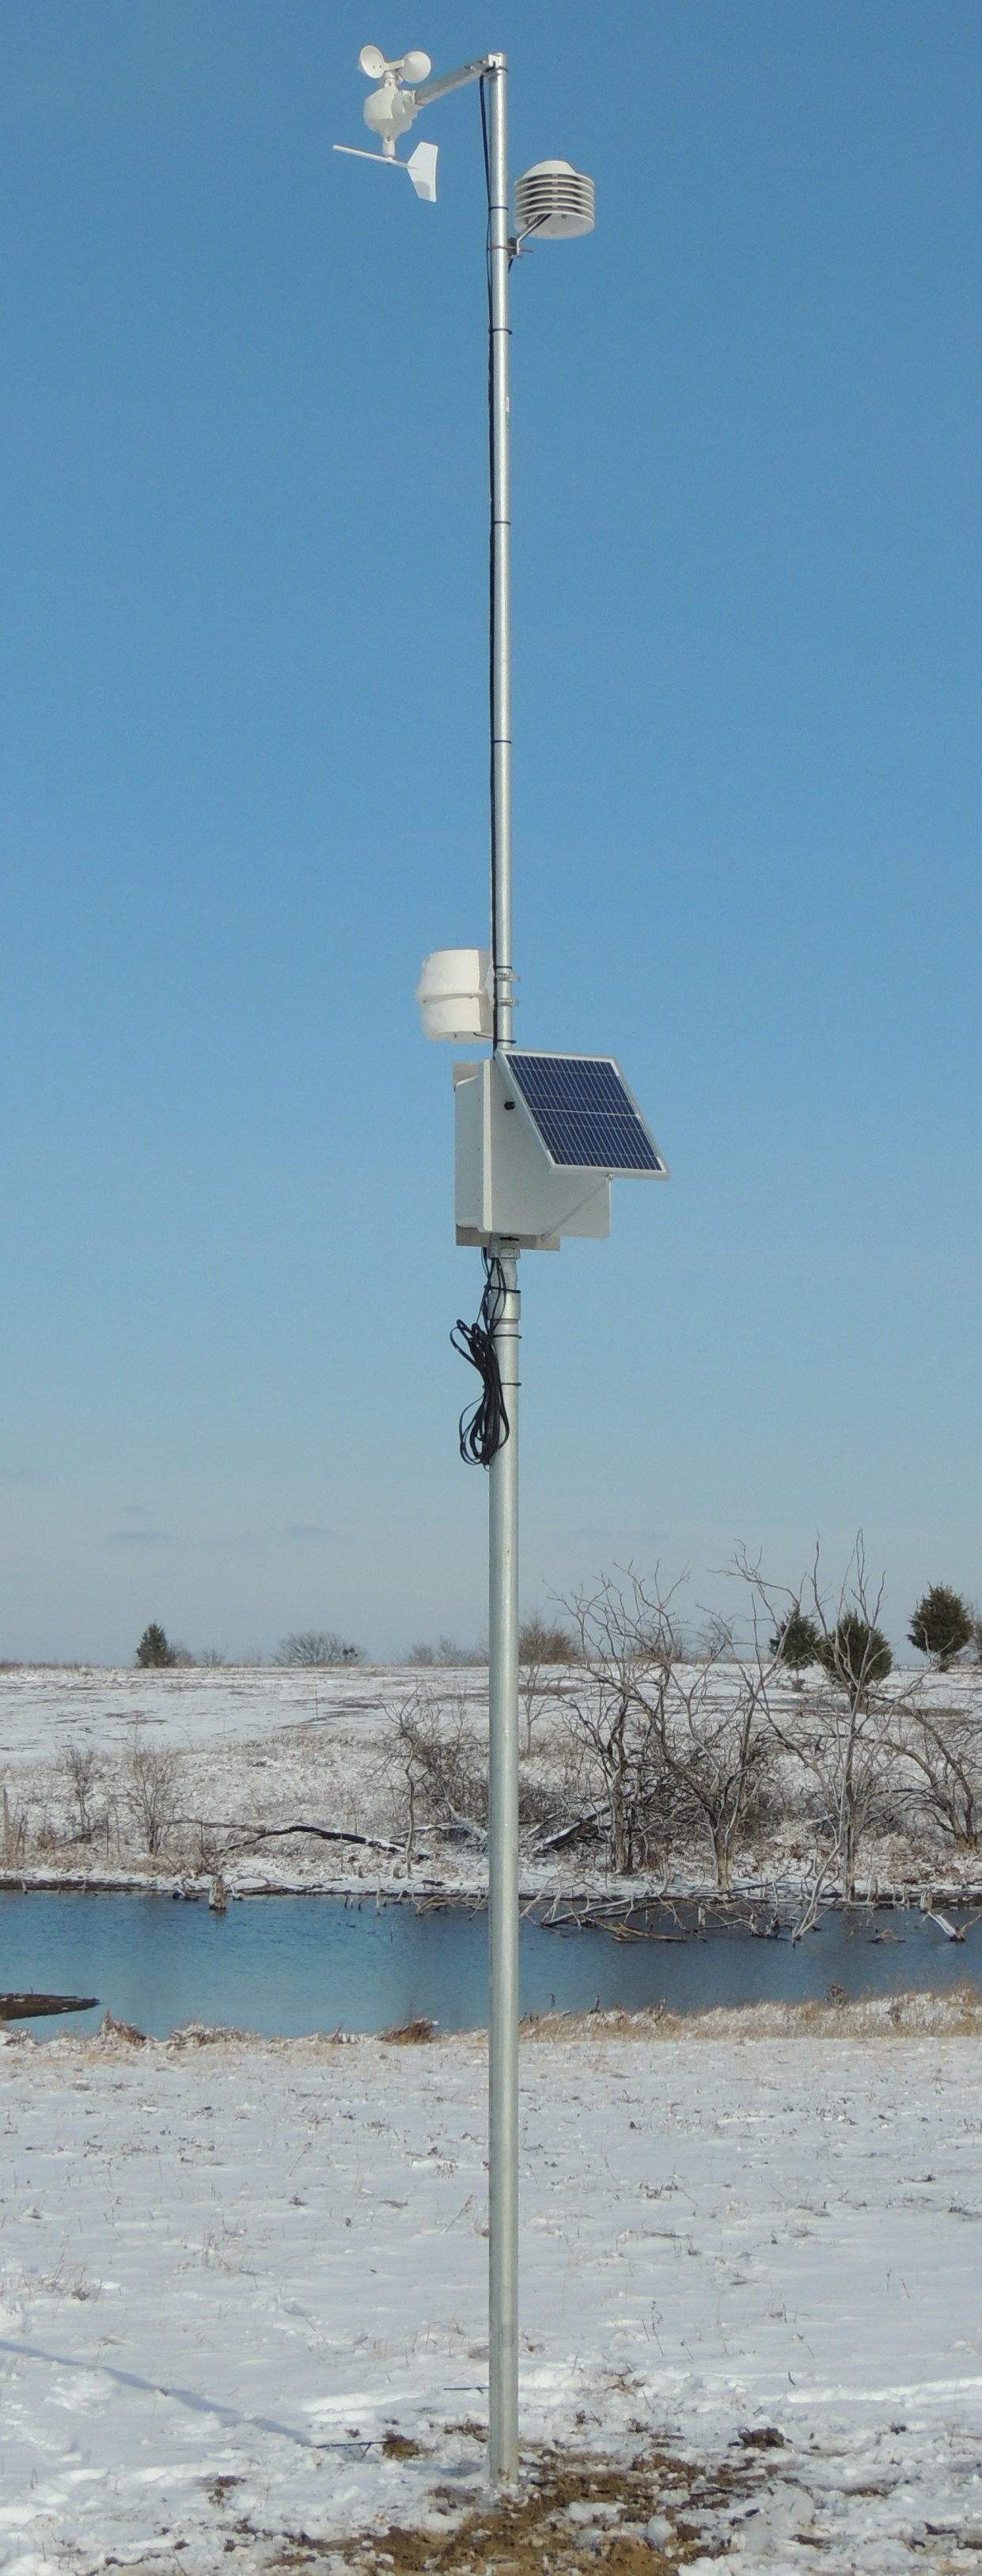
\includegraphics[height=5cm]{graphics/RWS-Snow.JPG}}\quad
  \subfloat[\$658\label{fig:c}\cite{Scientific2014}]
  {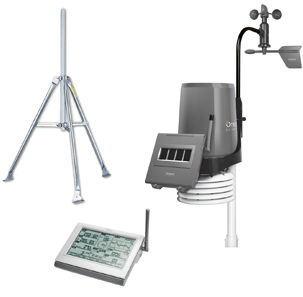
\includegraphics[height=3cm]{graphics/Oregon_Scientific_Pro_weather_system.PNG}}\quad
  \subfloat[\$595\label{fig:d}\cite{Davis2014}]
  {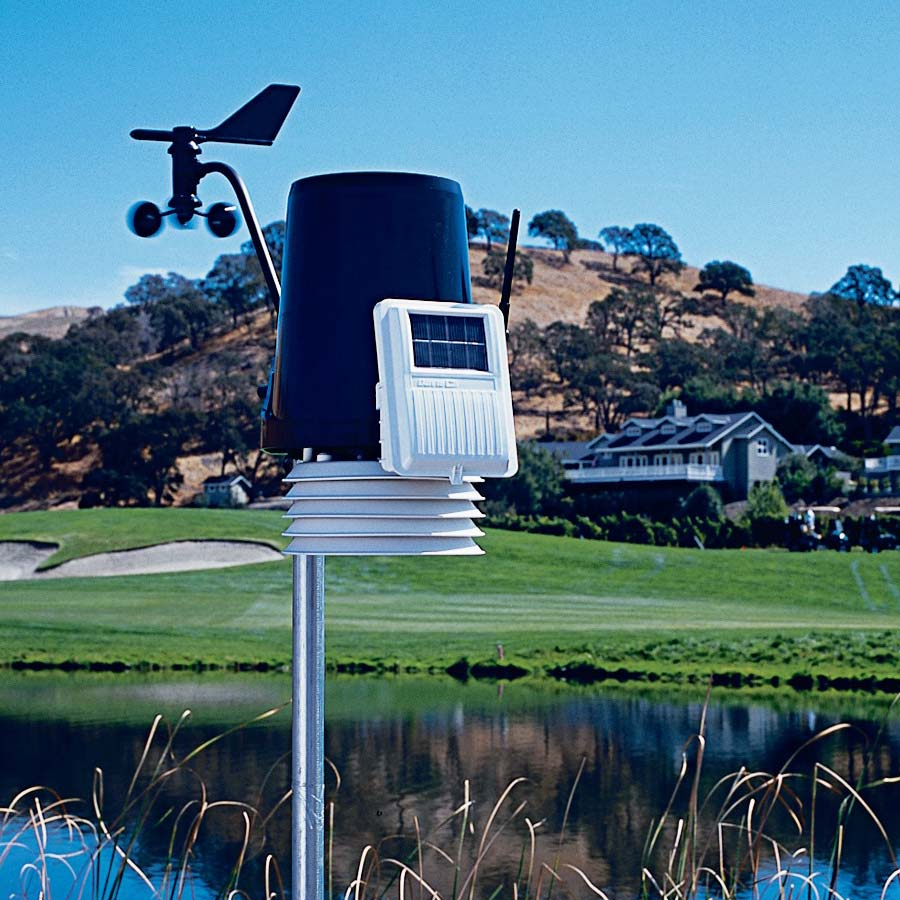
\includegraphics[height=3cm]{graphics/Davis_Vantage_Pro_2.JPG}}  
  \caption{Various price of weather stations}
  \label{fig:1}
\end{figure}
\end{frame}

\begin{frame}{Geolog Product}
	\begin{figure}
		\centering
		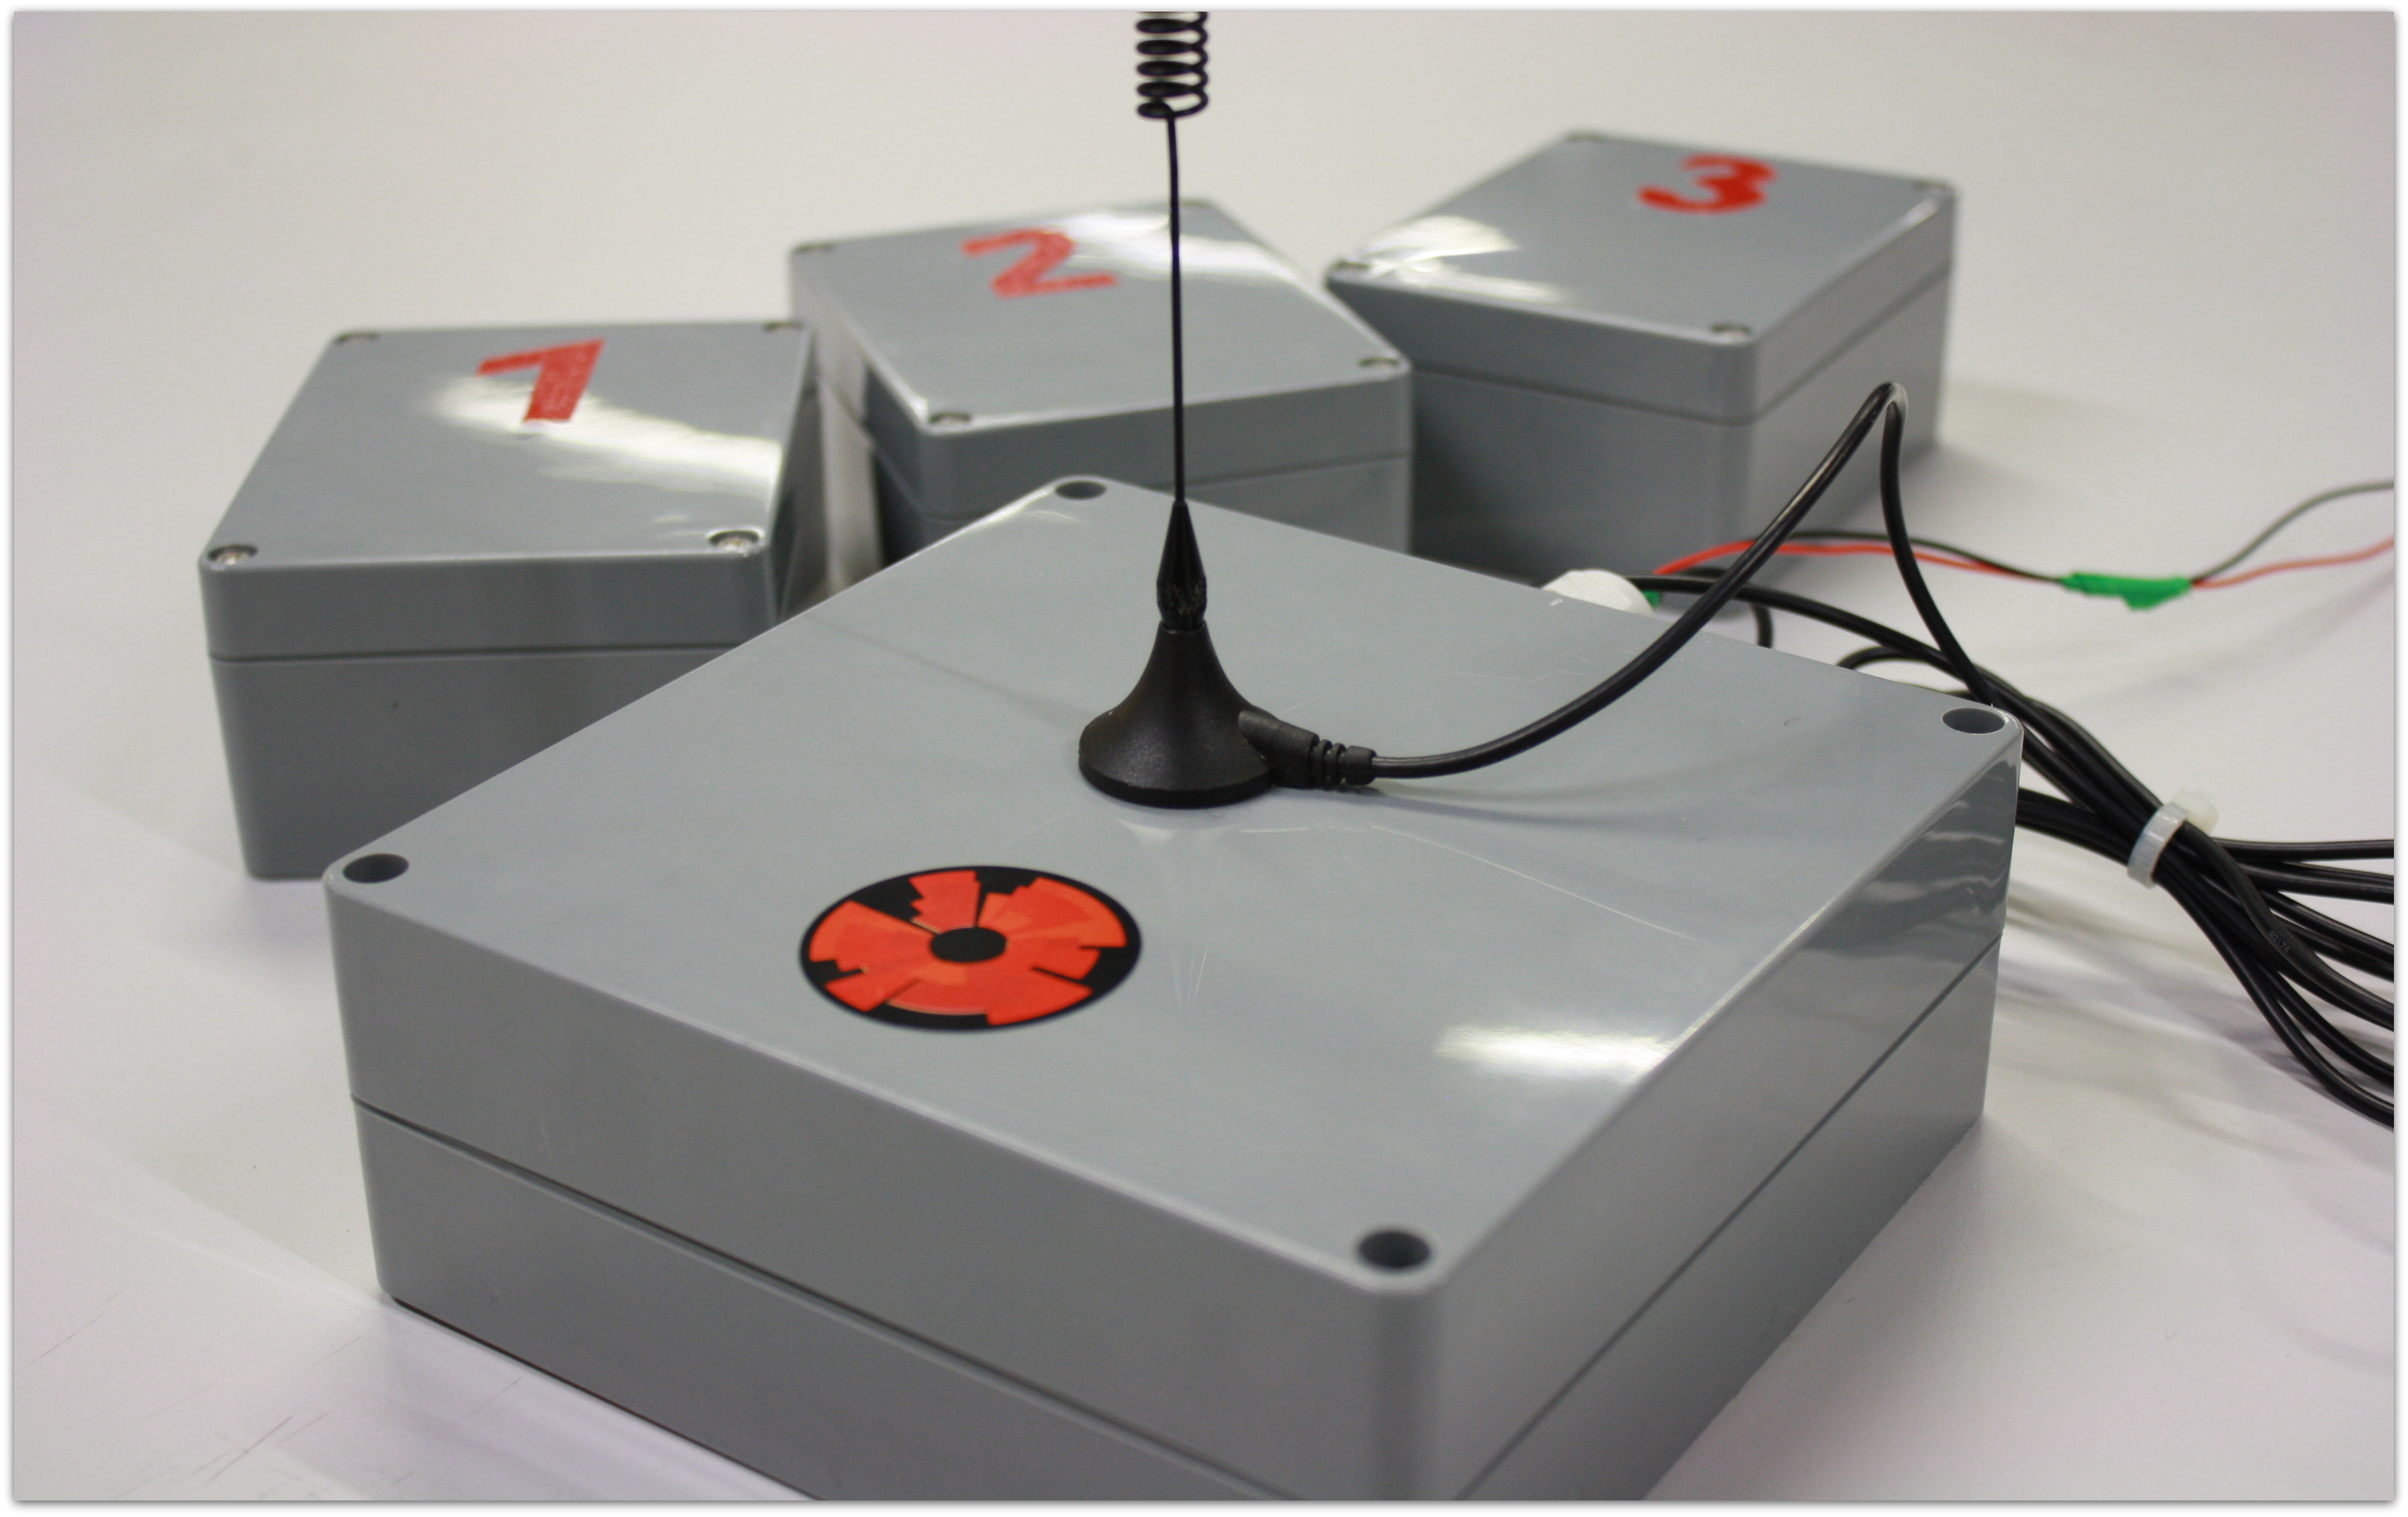
\includegraphics[height=6cm]{graphics/Field_pictures/Our_product.JPG}
		\caption{\$ 337.25 for 1x mother-base and 3x Wixel-sensors}
	\end{figure}
\end{frame}

\begin{frame}{Use case}
	\begin{itemize}
	\item Deployment of sensors
	\item Connect the sensors to communicators
		\begin{itemize}
		\item Wixel
		\item Xbee
		\item Any other wireless communicator
		\end{itemize}
	\item Position the main GeoLog module
	\item Connect to the Internet to see the incoming data
	\end{itemize}
	\begin{figure}
			\centering
	        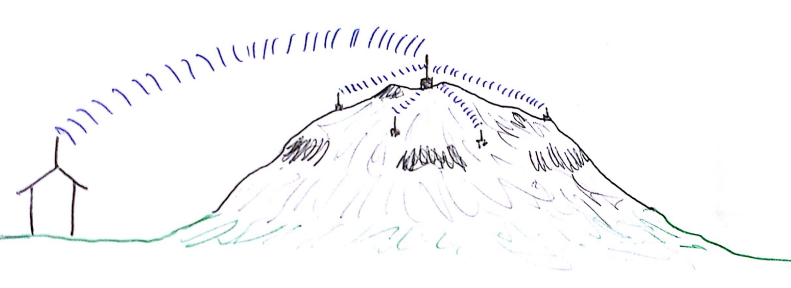
\includegraphics[height=3cm]{graphics/GeoLog.PNG}
	        \caption{Datalogging}
	\end{figure}

\end{frame}

\begin{frame}{Design: Layering}
\centering
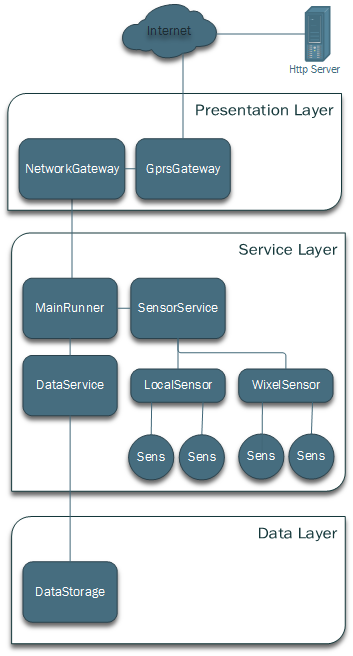
\includegraphics[height=7cm]{graphics/Layering.png}
%What are the pieces of your design (software, hardware, etc.)  and how
%do they work together?  Put some pictures here to help explain what is
%going on.  Remember to cite all pictures and text using BibTeX.  If you cited
%the textbook\cite{carryer2011IntroMechatronics}, that is what it would
%look like.
\end{frame}

\begin{frame}{Design: Module}
\centering
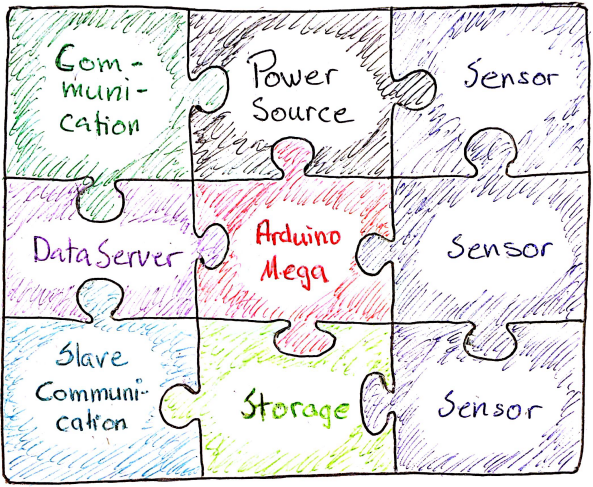
\includegraphics[height=7cm]{graphics/Puzzle.png}
%What are the pieces of your design (software, hardware, etc.)  and how
%do they work together?  Put some pictures here to help explain what is
%going on.  Remember to cite all pictures and text using BibTeX.  If you cited
%the textbook\cite{carryer2011IntroMechatronics}, that is what it would
%look like.
\end{frame}

\begin{frame}{Design: Software}
\centering
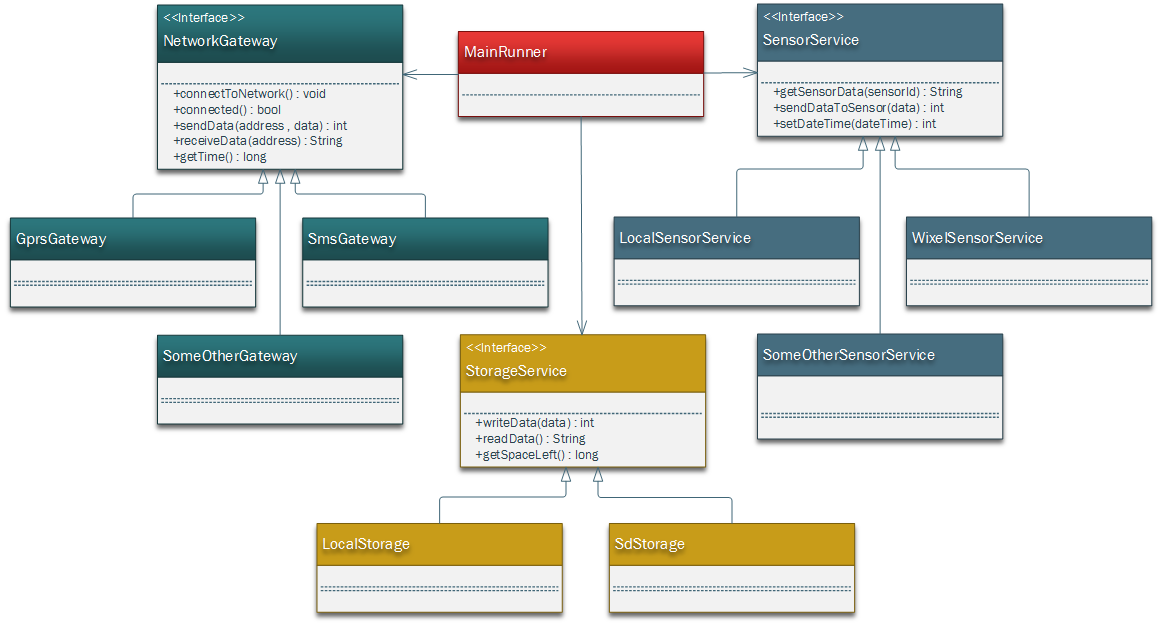
\includegraphics[width=11.5cm]{graphics/ClassDiagram.png}
\end{frame}

\begin{frame}{Design: Bill of materials (BOM) for mother station}
\begin{columns}[T]
	\begin{column}[T]{6cm}
		Main-base setup
		\begin{itemize} \small
		\item 1 x Arduino Mega (Model: 2560 R3 from Sparkfun) \$45.95
		\item 1 x GSM Module with shield  (Model: SM5100B from Sparkfun) \$99.95
		\item 1 x GSM Antenna \$ 40.00
		\item 1 x Battery pack \$ 2.00
		\item 1 x IP67 box \$ 25.00
		\item \textbf{\underline{Total cost of prototype \$ 212.90}} 
		\end{itemize}
	\end{column}
		\begin{column}[T]{4cm}
		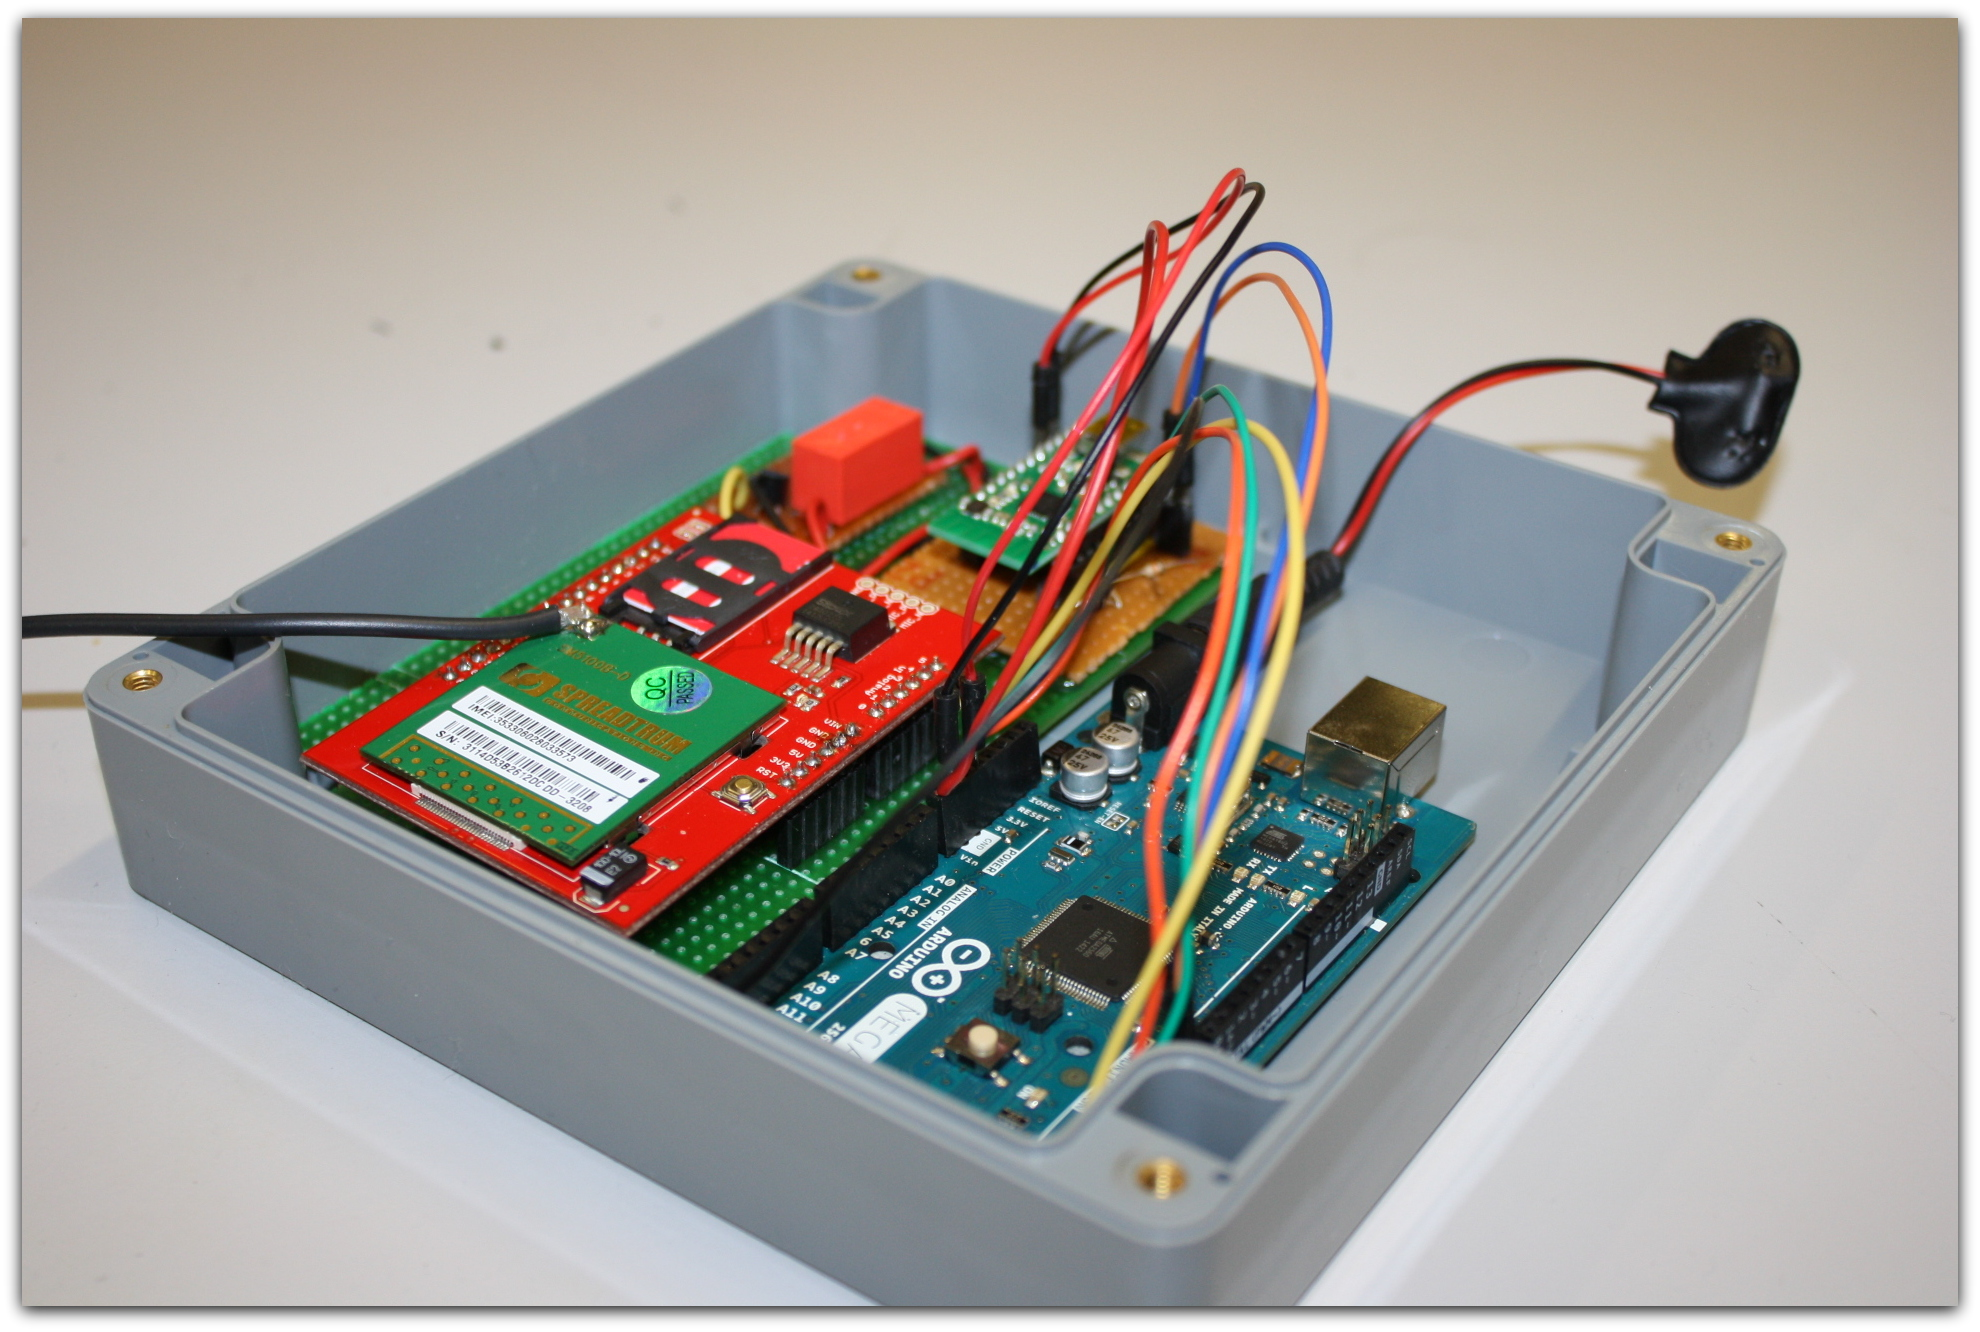
\includegraphics[height=2.7cm]{graphics/Field_pictures/Main_Open.JPG}\\
		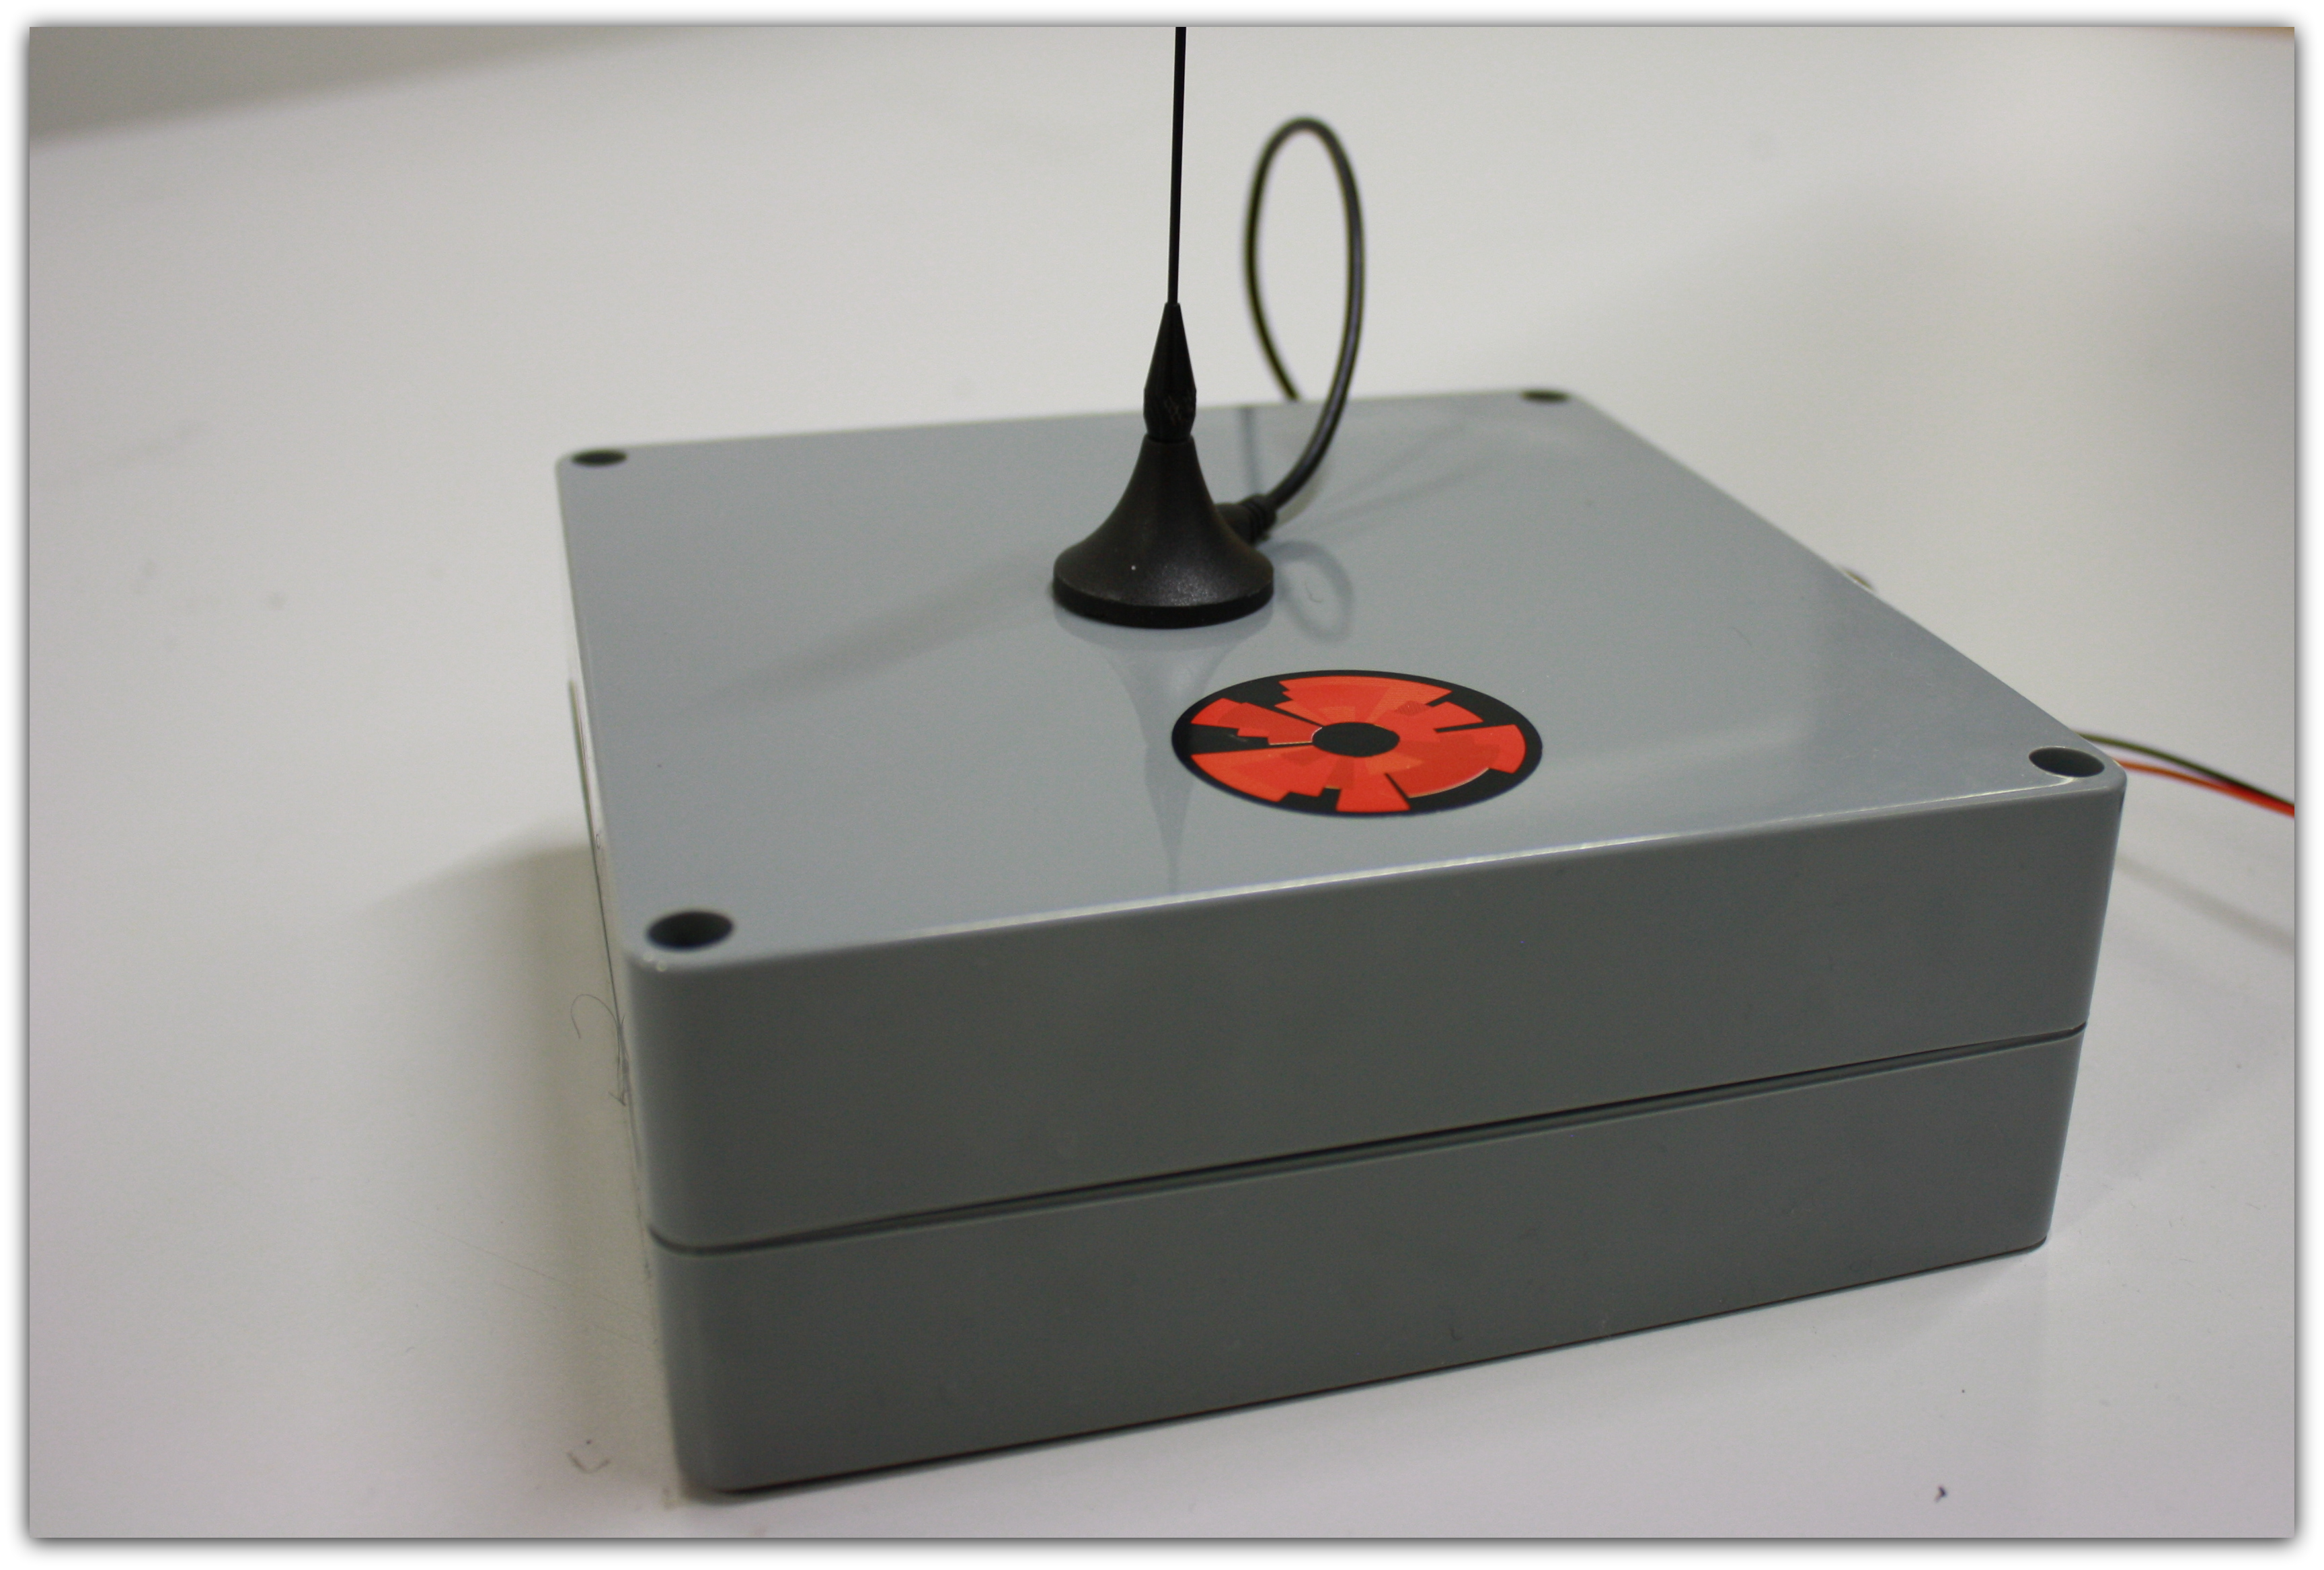
\includegraphics[height=2.7cm]{graphics/Field_pictures/Main_Close.JPG}
		\end{column}
\end{columns}
\end{frame}

\begin{frame}{Design: Bill of materials (BOM) Wixel-Sensor}
\begin{columns}[T]
	\begin{column}[T]{6cm}
		Wixel-base setup
		\begin{itemize} \small
		\item 1 x Wixel   (With CC2511F32 microc. from Sparkfun) \$19.95
		\item 1 x Temperature sensors (Model: TMP36 from Sparkfun) \$1.50
		\item 1 x Battery pack \$ 2.00
		\item 1 x IP67 box \$ 18.00
		\item \textbf{\underline{Total cost of prototype\$ 41.45}} 
		\end{itemize}
	\end{column}
		\begin{column}[T]{4cm}
		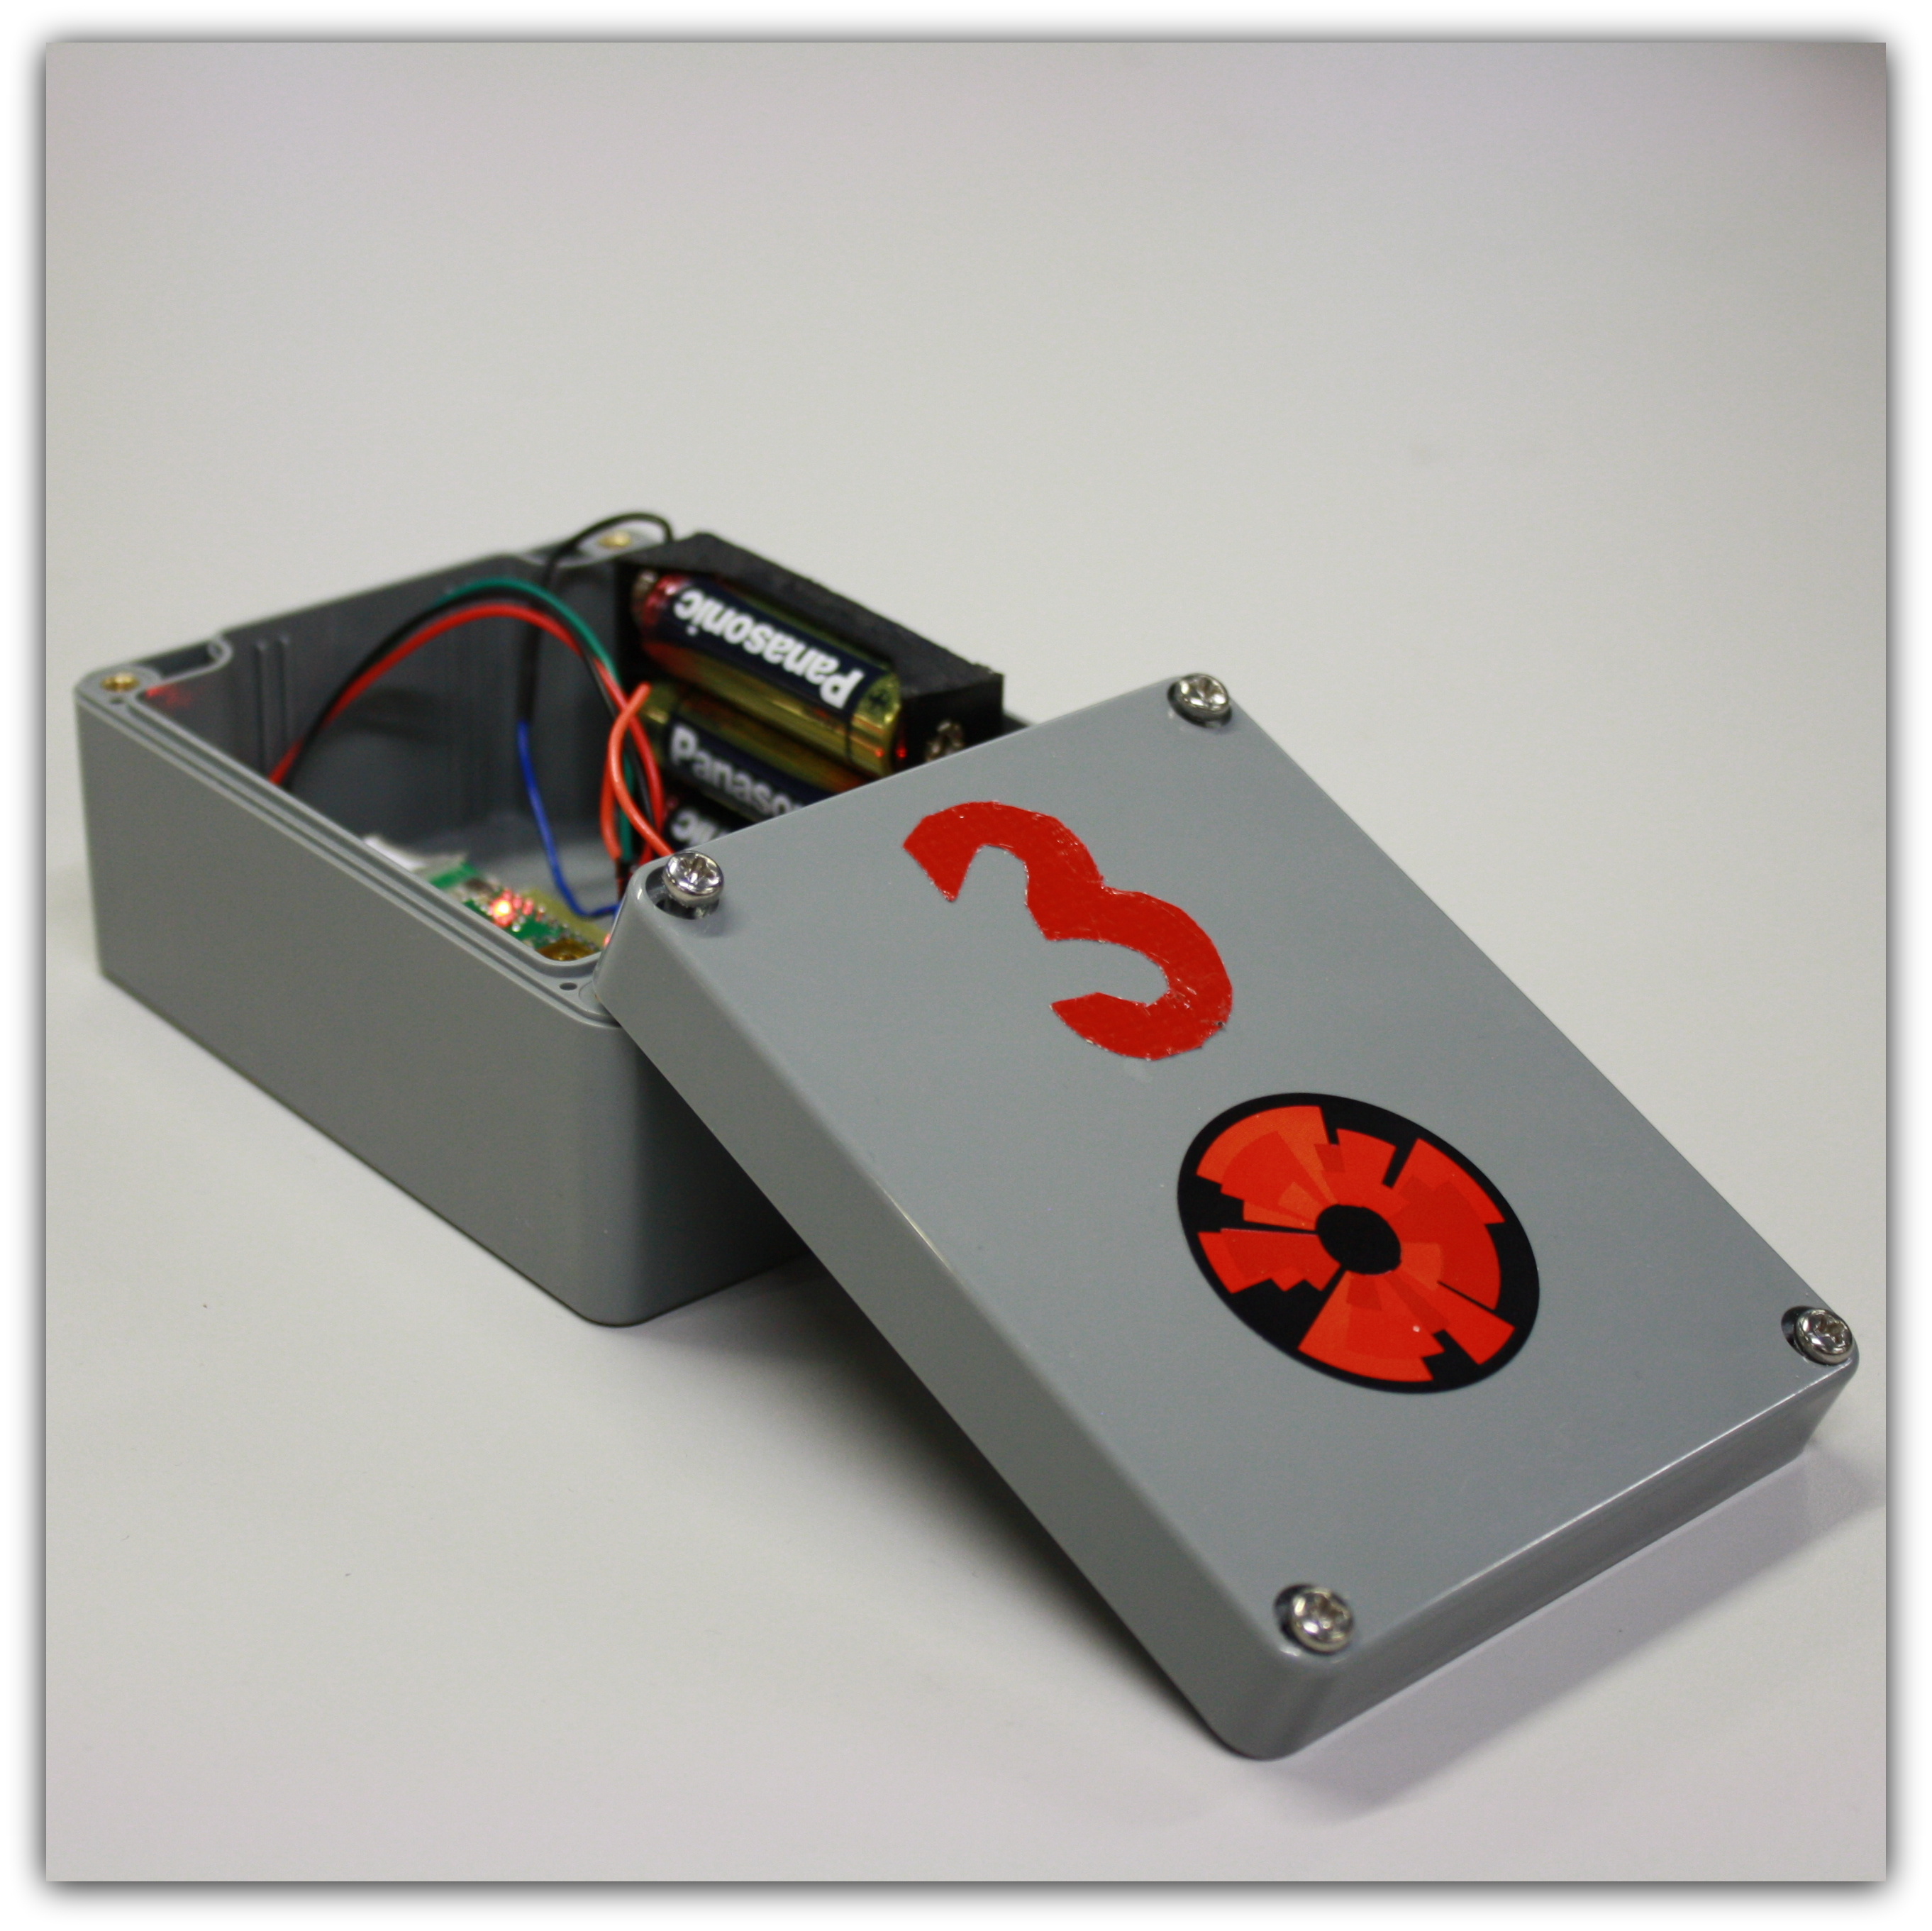
\includegraphics[height=4cm]{graphics/Field_pictures/Wixel_sensor.JPG}
		\end{column}
\end{columns}
\end{frame}

\begin{frame}{Status}
\centering
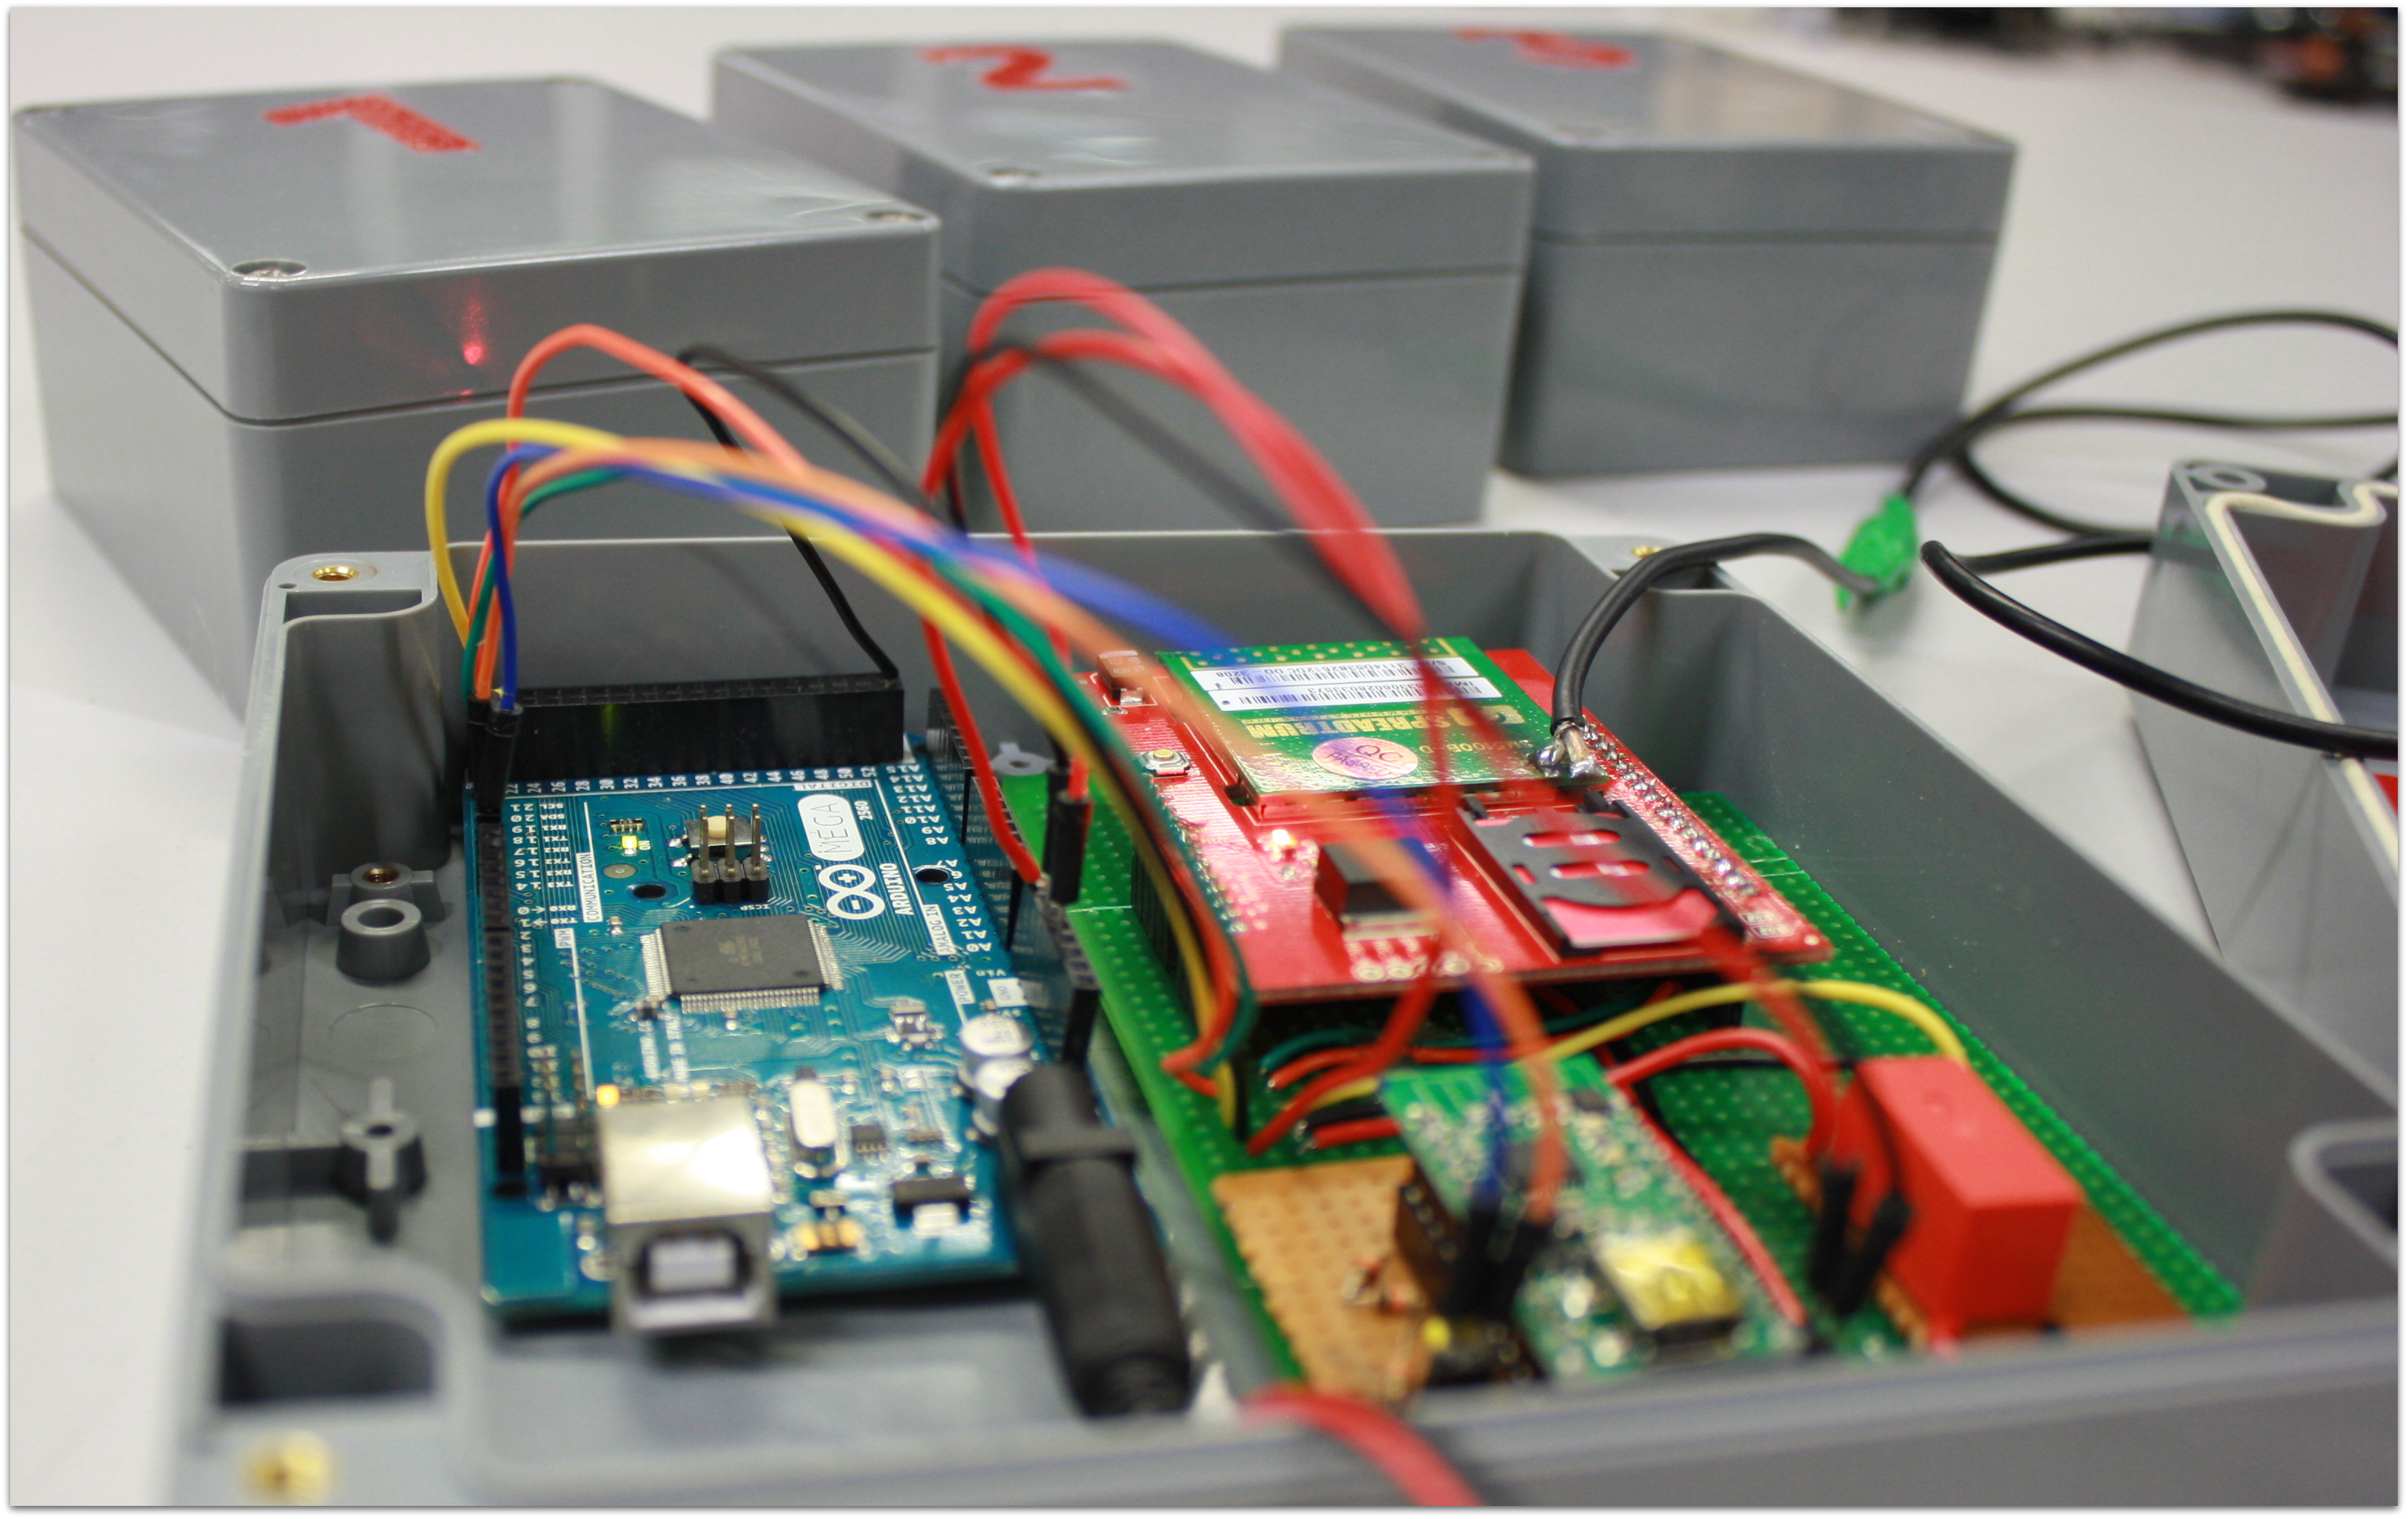
\includegraphics[width=11cm]{graphics/Field_pictures/Open_project.jpg}
\end{frame}

\begin{frame}{Performance}
\begin{columns}[T] % contents are top vertically aligned
     \begin{column}[T]{4cm} % each column can also be its own environment
		\begin{itemize}
		\item 4 kB accessible EEPROM
		\item 15 m wireless range on Wixel sensors
		\item GPRS/SMS on base station	 
		\item Unsatisfying energy consumption 
		\end{itemize}

		\end{column}
		\begin{column}[T]{5cm} % alternative top-align that's better for graphics
	     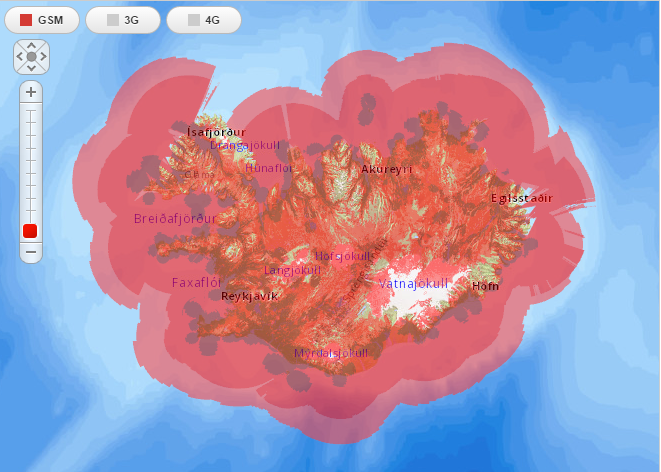
\includegraphics[height=4cm]{graphics/GSM_Coverage.PNG}
	     \cite{vodafone}
		\end{column}
	\end{columns}
\end{frame}

\begin{frame}{Interface}
\begin{columns}[T] % contents are top vertically aligned
     \begin{column}[T]{4cm} % each column can also be its own environment
		
		\begin{itemize}
		\item \href{http://sveinnel.com:5000/geolog}{HTTP API}
		\item \href{http://sveinnel.com:5000/geoblog}{GeoBlog interface}
		\end{itemize}
	\end{column}
     \begin{column}[T]{5cm} % alternative top-align that's better for graphics
          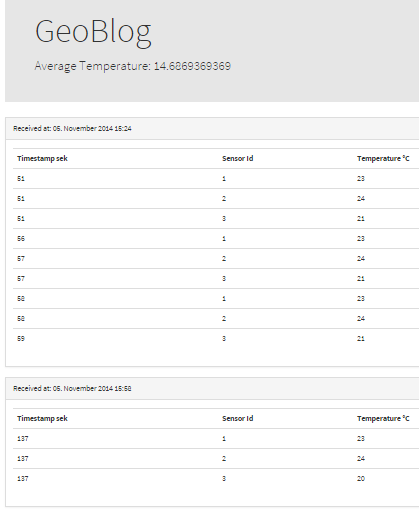
\includegraphics[height=6cm]{graphics/GeoBlog.png}
     \end{column}
     \end{columns}
%What have you done?  What is the current state?  Is there any interesting/hard problems
%that need to be solved?  How are you going to solve them?
\end{frame}

\begin{frame}{Field test}
\centering
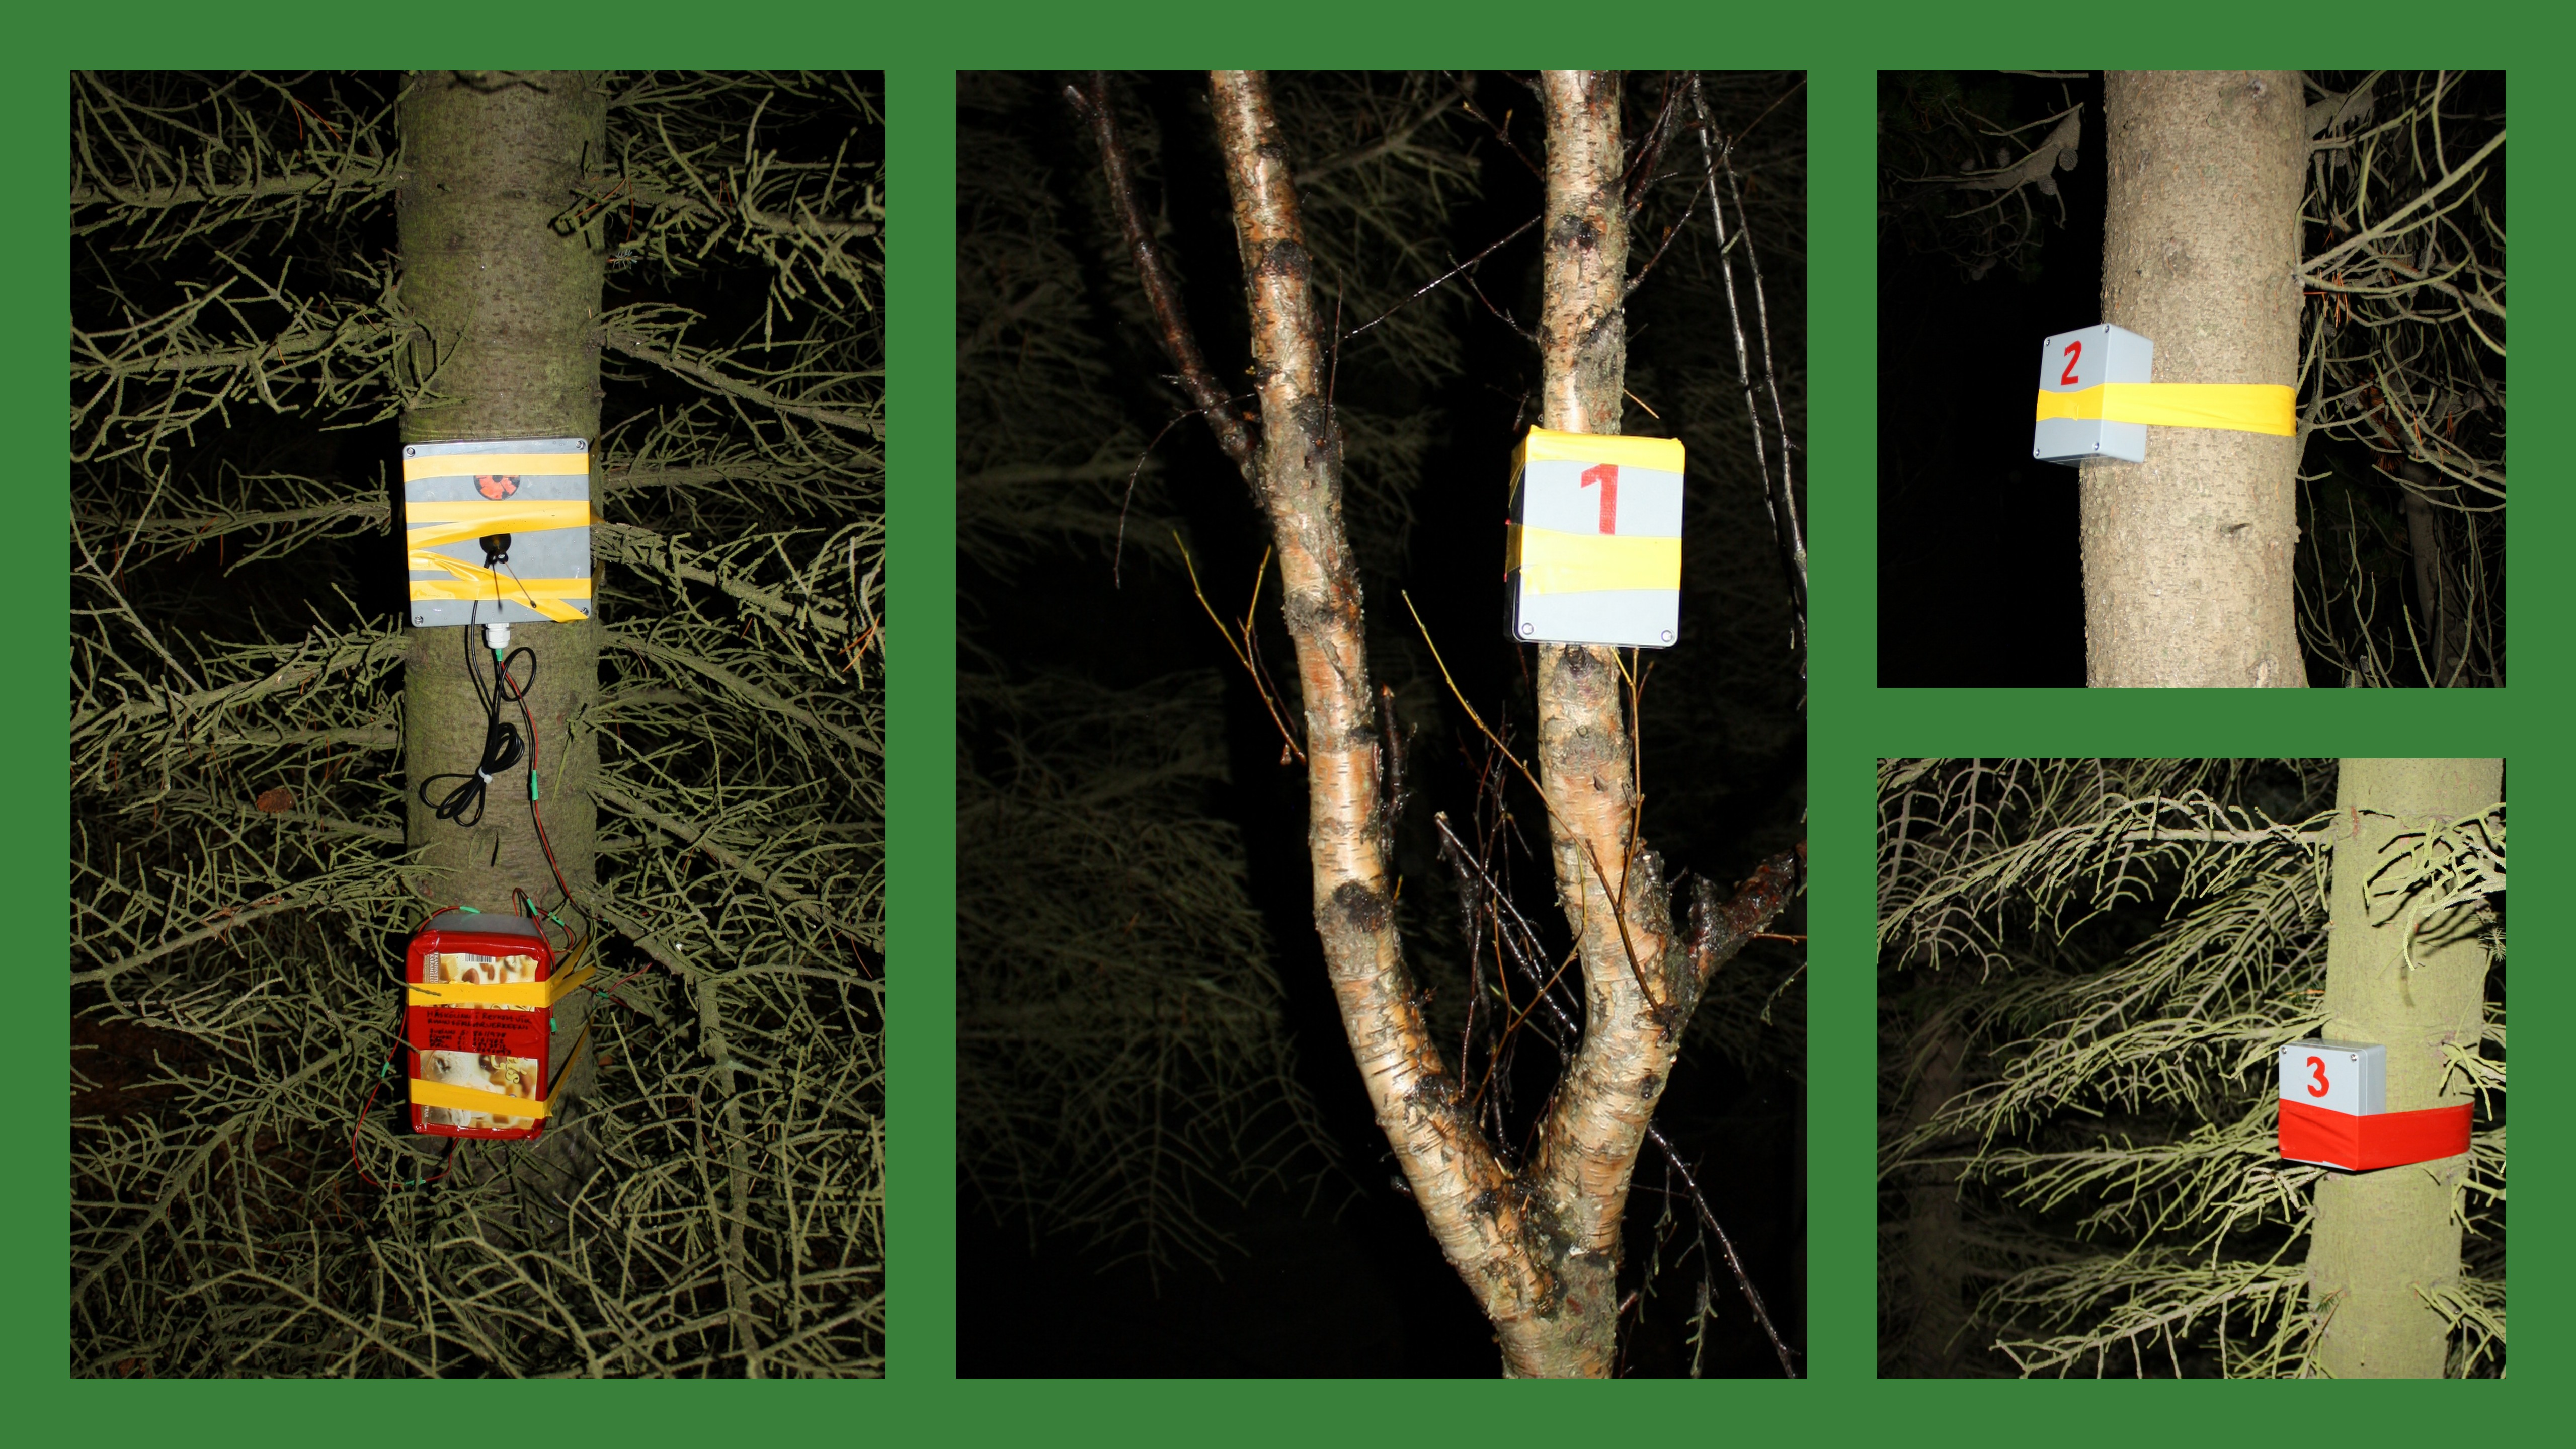
\includegraphics[width=11cm]{graphics/Field_pictures/Field_DataLogger.jpg}
\end{frame}

\begin{frame}{Next steps and future possibilities}
%What is left to be done?  This should be broken down by the time remaining in class.
\begin{columns}[T]
	\begin{column}[T]{7cm}
		\begin{itemize}
		\item Continuing field test
		\item Improve user-interface
		\item Implement other communication modules
			\begin{itemize}
			\item Iridium, Radio ...
			\end{itemize}
		\item Merge to Andy's data logger
		\item Improve energy consumption
		\item Implement other energy sources 
			\begin{itemize}
			\item Solar, Wind ...
			\end{itemize}
		\end{itemize}
	\end{column}
	\begin{column}[T]{4cm}
	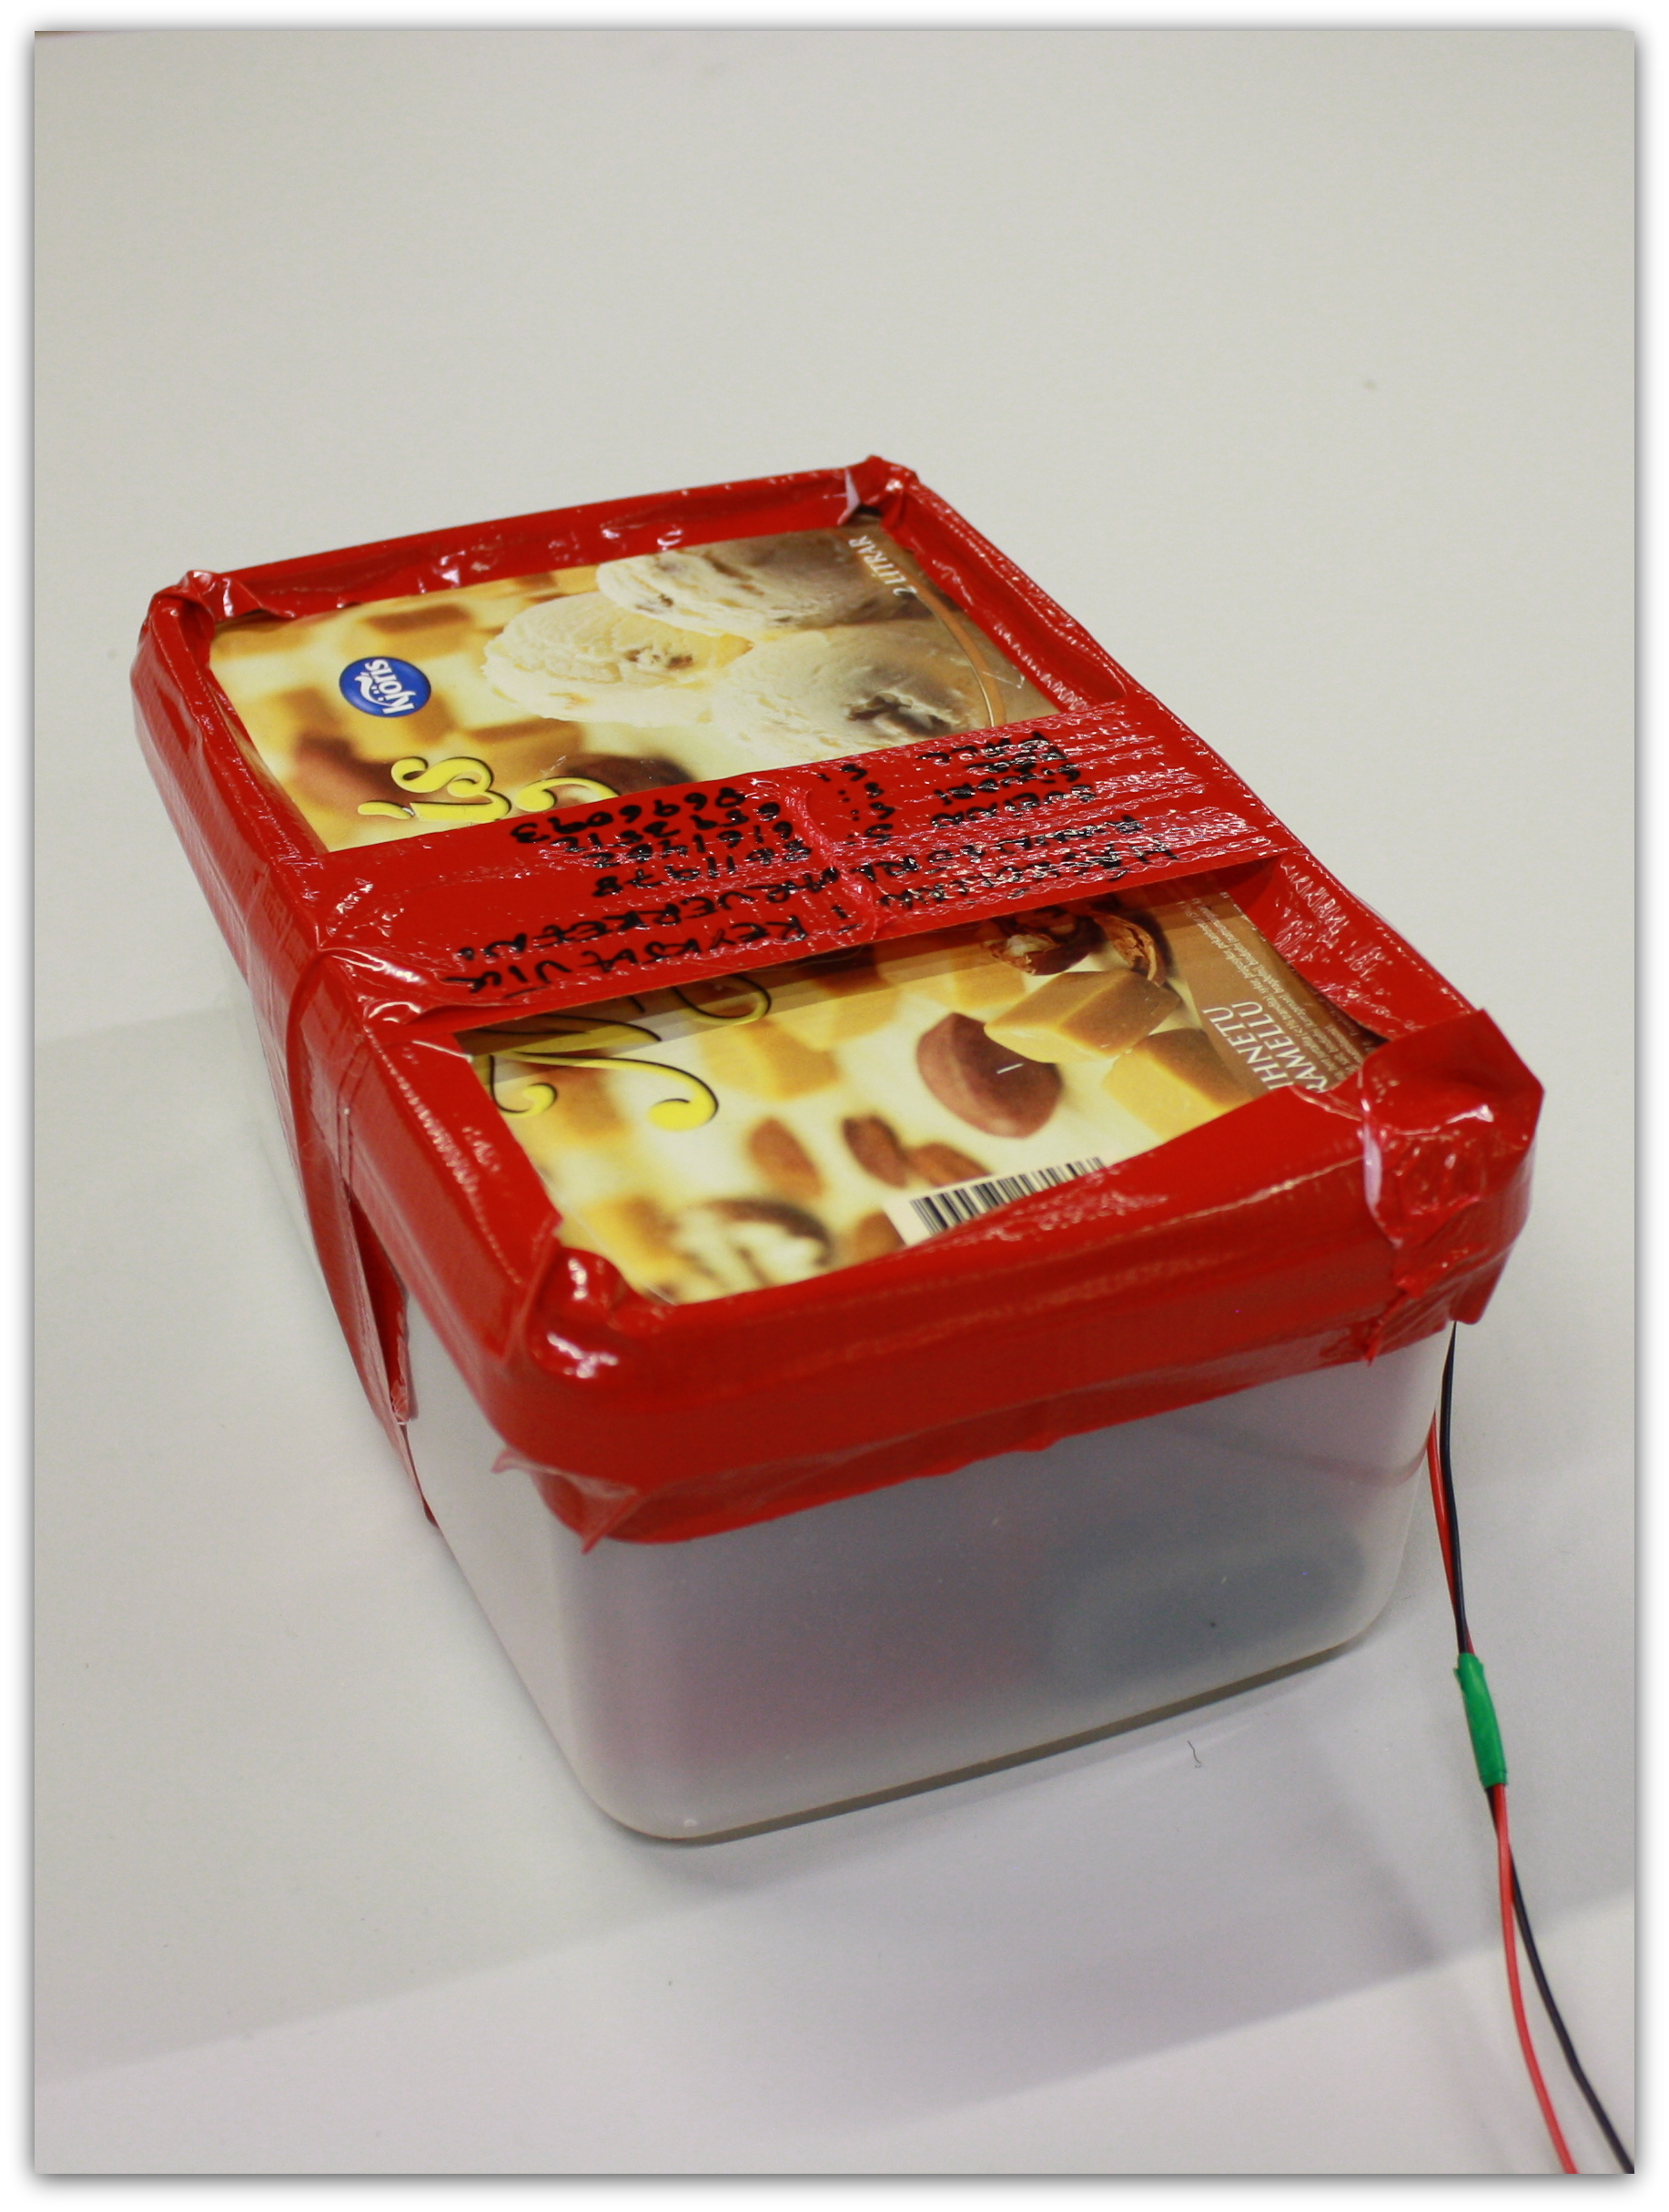
\includegraphics[height=4cm]{graphics/Field_pictures/Power.jpg}
	\end{column}
\end{columns}
\end{frame}

\begin{frame}{Summary}
\begin{columns}[T]
	\begin{column}[T]{6cm}
		\begin{itemize}
		\item Bee hive design
		\item Modular software architecture
		\item HTTP REST API
		\item Affordable
		\item Open source
		\item Highly modifiable
		\end{itemize}
	\end{column}
	\begin{column}[T]{4cm}
	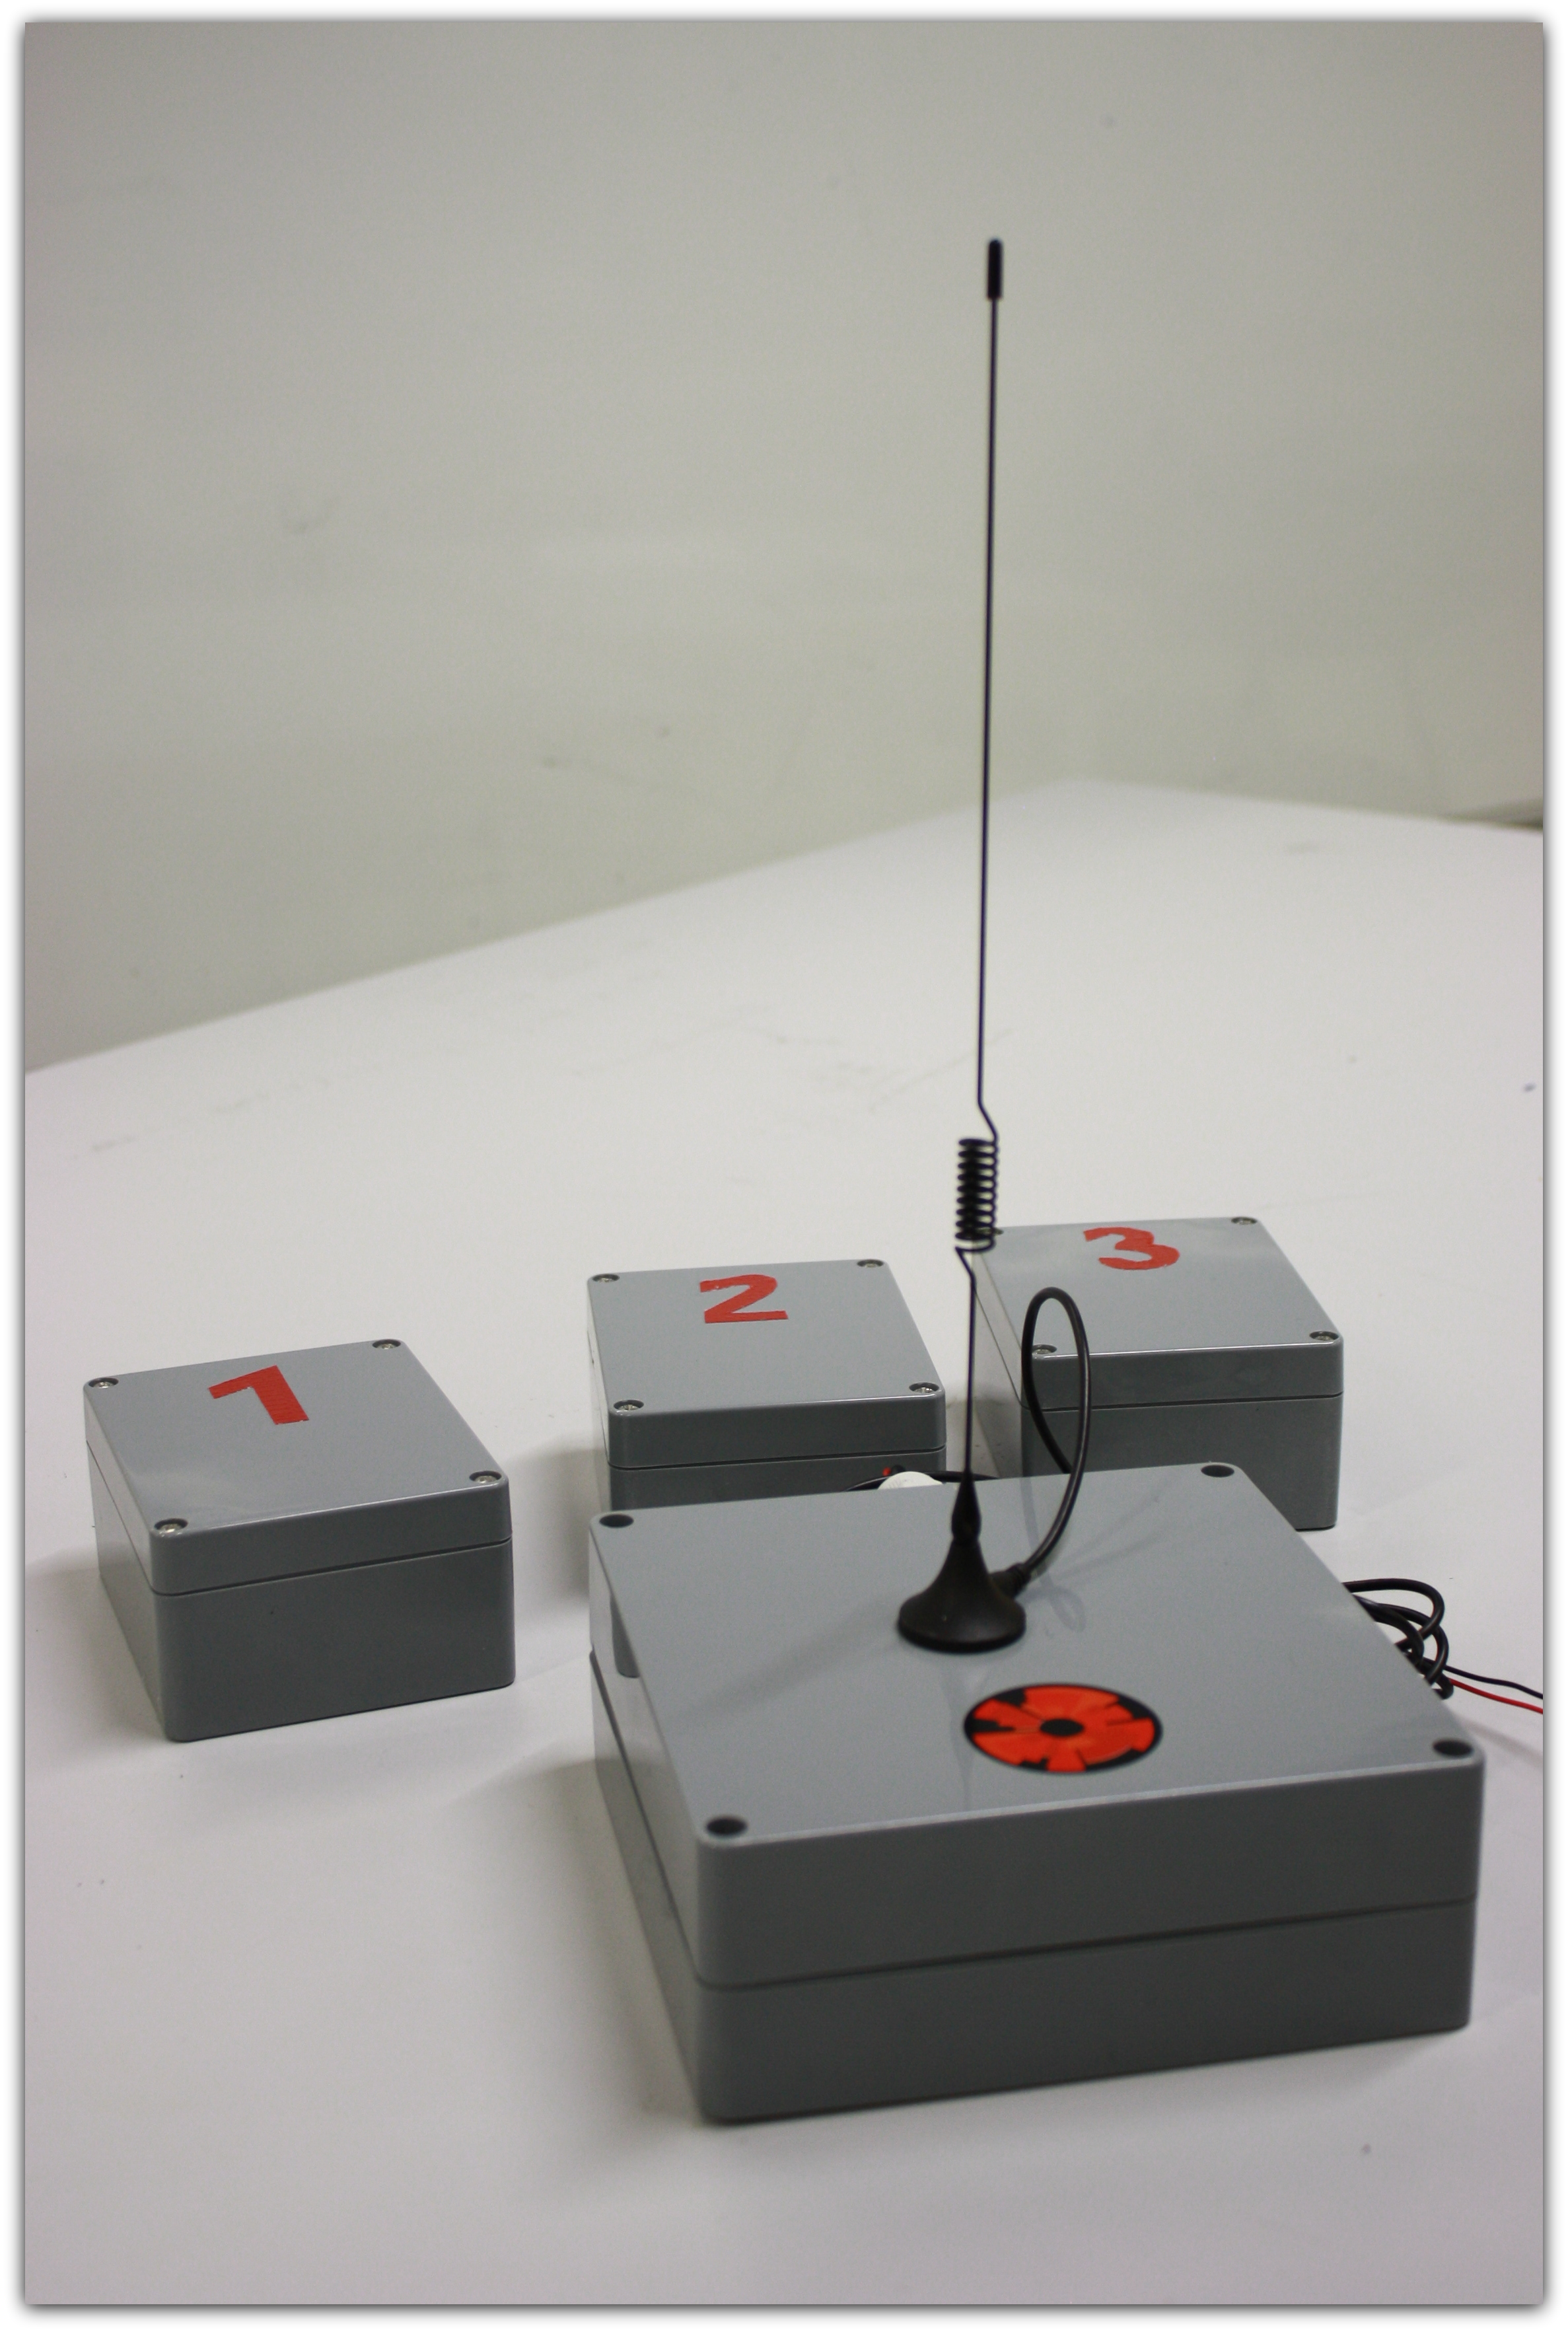
\includegraphics[height=5cm]{graphics/Field_pictures/Main_and_Wixels.JPG}
	\end{column}
\end{columns}
\end{frame}

\begin{frame}{References}
Thank you for your time.
Questions?
\bibliographystyle{IEEEtran}
{\tiny \bibliography{references}}
\end{frame}

\end{document}
